\documentclass[letterpaper,10pt,oneside,final,onecolumn]{article}

\usepackage[utf8x]{inputenc}
\usepackage{amsmath}
\usepackage{amsfonts}
\usepackage{amssymb}
\usepackage{amsthm}
\usepackage[canadian]{babel}
\usepackage[retainorgcmds]{IEEEtrantools}
\usepackage{mathrsfs}
\usepackage[pdftex]{graphicx}
\usepackage{algorithm}
\usepackage{algpseudocode}
\usepackage{longtable}
\usepackage{listings}
\usepackage{tikz}
\usepackage{graphicx}

% Verbatim language configurations
\lstset{
	language=SQL,
	basicstyle=\scriptsize\ttfamily,
	tabsize=2,
	showspaces=false,
	showtabs=false,
	showstringspaces=false,
	identifierstyle=\color{gray},
	keywordstyle=\color{blue},
	stringstyle=\color{cyan},
	commentstyle=\color{green},
	morekeywords={IIF,UCase,RTrim,LTrim,IS,IsNumeric,ABS,Format}
}

% Table configurations
\renewcommand{\arraystretch}{1.5}

\author{Aaron Sheldon}
\title{Pipeline Accident Probability Estimators}
\date{\today}

\begin{document}
	\maketitle
	\begin{abstract}
		In this letter we derive the maximum likelihood estimators of the parameters of a compound Poisson process, and the asymptotic variance of the estimators.
		Using the maximum likelihood estimators of the parameters, we derive the maximum likelihood estimator of the forecast probability of future pipeline accidents, with confidence intervals; as a function of forecast time, forecast pipeline length, and forecast spill volume.
		To illustrate the results we apply the derived maximum likelihood estimators to a data set of historical pipeline accidents, to forecast the probability of future pipeline accidents. 
	\end{abstract}

	\section{Introduction}\label{introduction}
	Much as the probability of precipitation in daily weather forecasts can be statistically constructed through comparison with historical weather records, the probability of future pipeline accidents can statistically constructed from historical pipeline accident records.
	Our goal in this letter is to forecast the probability of future pipeline accidents, with confidence intervals, as a function of forecast time, forecast pipeline length, and forecast spill volume.
	We will proceed in 5 steps:
	First, making the fewest mechanistic assumptions possible, we will propose a joint distribution for the occurrence, and size of pipeline accidents.
	Second, we will derive the maximum likelihood estimators for the parameters of the joint distribution.
	Third, we will propose an estimator for the probability of future pipeline accidents, arguing from the properties of the proposed joint distribution.
	Forth, using the Fisher information matrix, we will derive the asymptotic variance of the proposed estimator, and hence the confidence intervals.
	Finally, we will apply the estimator to historical pipeline accident data available from the \textit{United States of American Department of Transportation \textbf{P}ipeline and \textbf{H}azardous \textbf{M}aterials \textbf{S}afety \textbf{A}dministration}.

	\section{Notation}\label{notation}
	In this letter we will denote single random variables by upper case letters $N, X, Y$; and their stochastic process analogues by the super-scripted bracket of the filtration index $s$, so that $N^{\left(s\right)}, X^{\left(s\right)}, Y^{\left(s\right)}$ are stochastic processes.
	Specific non-random scalar values will be denoted by lower case letters $n, x, y$.
	The distributions will be parametrized by lower case Greek letters $\lambda, \rho$, and their maximum likelihood estimation from the stochastic random variables will be denoted with the hat $\hat{\lambda}, \hat{\rho}$. 
	The common statistical measure theoretic functionals of probability measure, expectation, indicator, variance, and covariance will be denoted by vertical barred upper case letters $\mathbb{P}, \mathbb{E}, \mathbb{I}$.
	We will make use of the concise summation notation 
	\begin{IEEEeqnarray*}{rCl}
		s_{n:m} & = & \sum_{i=n}^m s_i
	\end{IEEEeqnarray*}
	for any sum of countably indexed values $s_i$, that may be either non-random scalar values, or random variables.

	\section{Joint Distribution}\label{joint-distribution}
	As noted in the review by Gunton and Broadbent, the number of pipeline accidents in pipeline length $l$, and service usage time $t$, has been established to be a Poisson process $N^{\left(lt\right)}$
	\begin{IEEEeqnarray*}{rCl}
		\mathbb{P} \left[N^{\left(lt\right)} = n \right]
			& = & \frac{\left( l t \lambda \right)^n}{n!} e^{- l t \lambda}
	\end{IEEEeqnarray*}
	where $\lambda$ is the accident rate per unit $lt$ of the product of pipeline length and service usage time.
	Our first assumption, in this letter, will be that the accidents follow a Poisson process; this explicitly requires that the accidents are rare events, which are stationary, and homogeneous in pipeline length $l$, and service usage time $t$.

	The second assumption we will carry throughout this letter is that the accident volumes $X^{\left(i\right)}$ are independently, and identically distributed.
	Because our goal is to forecast the probability of accidents of at least some minimal volume $b_r$ we can dispense with making explicit assumption on the parametric distribution of accident volumes.
	Instead, we will estimate the empirical probability distribution of accidents volumes occurring in $k$ empirical bins, which we define by the boundary points $0 = b_0 < b_1 < \cdots < b_{k-1} < b_k = \infty$.
	
	We can empirically approximate the distribution of the volume $X^{\left(i\right)}$ of the $i$ accident with respect to the boundaries $b_j$
	\begin{IEEEeqnarray*}{rCl}
		\rho_j & = & \mathbb{P}\left[b_{j-1} \le X < b_j \right]
	\end{IEEEeqnarray*}
	Where the parameters $\rho_j$ estimate the corresponding probabilities that the volume of a single accident is in the bin $\left[b_{j-1}, b_j \right)$.
	It follows, from the summation normalization of probabilities, that the parameter $\rho_k$, which estimates the probability that the volume of a single accident will be in largest spill volume bin, is given by $\rho_k = 1 - \rho_{1:k-1}$.

	By the independence of the individual accident volumes $X^{\left(i\right)}$, the cumulative volume spilled of all accidents occurring in pipeline length and service usage time $lt$ is a compound Poisson process over a continuous filtration indexed by $lt$
	\begin{IEEEeqnarray*}{rCl}
		Y^{\left(lt\right)} & = & \sum_{i = 1}^{N^{\left(lt\right)}} X^{\left(i\right)}
	\end{IEEEeqnarray*}
	In this compound Poisson process, the product of pipeline length and service usage time $lt$ takes the place of the sample count $n$ found in the theory of sampling distributions.
	We can then apply the theory of maximum likelihood estimation; replacing the asymptotic limit of large sample size $n \rightarrow \infty$ over a countable filtration, with the asymptotic limit of large product of pipeline length and service usage time $lt \rightarrow \infty$ over a continuous filtration.

	The joint distribution of the compound Poisson process $Y^{\left(lt\right)}$ is defined with respect to the random variables that count the number of accidents occurring in volume bin $\left[b_{j-1}, b_j\right)$, within pipeline length and service usage time $lt$.
	\begin{IEEEeqnarray*}{rCl}
		N_j^{\left(lt\right)} & = & \sum_{i = 1}^{N^{\left(lt\right)}} \mathbb{I} \left[ b_{j-1} \le X^{\left(i\right)} < b_j \right]
	\end{IEEEeqnarray*}
	The joint distribution of the sub-counting processes $N_j^{\left(lt\right)}$ is then the product of the Poisson distribution of the total number of accidents $N_{1:k}^{\left(lt\right)} = N^{\left(lt\right)}$ with the multinomial distribution of accident counts in volume bins $\left[b_{j-1}, b_j\right)$
	\begin{IEEEeqnarray*}{rCl}
		\IEEEeqnarraymulticol{3}{l}{\mathbb{P}\left[N_1^{\left(lt\right)} = n_1, \dots , N_k^{\left(lt\right)} = n_k \right]} \\
			\qquad & = & \frac{\left( l t \lambda \right)^{n_{1:k}}}{n_{1:k}!} e^{- l t \lambda} \binom{n_{1:k}}{n_1 \cdots n_k}\rho_1^{n_1} \cdots \left(1 - \rho_{1:k-1} \right)^{n_k}
	\end{IEEEeqnarray*}
	where the counts $n_j$ are the observed accident frequencies.

	\section{Parameter Estimation}\label{parameter-estimation}
	From the joint distribution of the compound Poisson process, through the standard techniques of differential calculus, we can derive the maximum likelihood estimators of the parameters for the accident rate $\lambda$ per unit product of pipeline length and service usage time, and the empirical probabilities $\rho_i$ of an accident of having a spill volume in bin $\left[b_{j-1}, b_j\right)$.
	Assuming the accident sub-counting process $N_j^{\left(lt\right)}$, the maximum likelihood estimator $\hat{\lambda}$, of the accident rate $\lambda$ is 
	\begin{IEEEeqnarray*}{rCl}
		\hat{\lambda} & = & \frac{N_{1:k}^{\left(lt\right)}}{l t}
	\end{IEEEeqnarray*}
	Likewise, from the same assumption, the maximum likelihood estimators $\hat{\rho_j}$, of the empirical probabilities $\rho_j$ are
	\begin{IEEEeqnarray*}{rCl}
		\hat{\rho}_j & = & \frac{N_j^{\left(lt\right)}}{N_{1:k}^{\left(lt\right)}}
	\end{IEEEeqnarray*}
	In this compound Poisson process, the maximum likelihood estimators are also unbiased estimators of the parameters.
	The asymptotic covariance of the maximum likelihood estimators is given by
	\begin{IEEEeqnarray*}{rCl}
		\mathbb{C}ov \left[\hat{\lambda}, \hat{\rho}_1, \dots , \hat{\rho}_{k-1} \right] 
		& = &
		\begin{bmatrix}
			\frac{\lambda}{lt} & \ldots                                            & 0      & \ldots \\
			\vdots             & \frac{\rho_1 \left(1 - \rho_1\right)}{lt \lambda} & \ldots & - \frac{\rho_1 \rho_{k-1}}{lt \lambda} \\
			0                  & \vdots                                            & \ddots & \vdots \\
			\vdots             & - \frac{\rho_1 \rho_{k-1}}{lt \lambda}            & \ldots & \frac{\rho_{k-1} \left(1 - \rho_{k-1}\right)}{lt \lambda}
		\end{bmatrix}
	\end{IEEEeqnarray*}
	The inverse dependence on the product of the pipeline length and service usage time $lt$, demonstrates that the estimators are consistent in $lt$.
	Specifically, we have that $\hat{\lambda} \rightarrow \lambda$ and $\hat{\rho}_j \rightarrow \rho_j$ as $lt \rightarrow \infty$, because $\mathbb{C}ov \left[\hat{\lambda}, \hat{\rho}_1, \dots , \hat{\rho}_{k-1} \right] \rightarrow 0$ as $lt \rightarrow \infty$.

	\section{Forecast Estimation}\label{forecast-estimation}
	Omitting the details of the derivation, the maximum likelihood estimators of the parameters $\hat{\lambda}$ and $\hat{\rho}_j$ can be used to estimate the forecast probability $H_r^{\left(\tilde{l} \tilde{t} \right)}$ of at least 1 accident with a volume of at least $b_r$, in a forecast pipeline length of $\tilde{l}$, and forecast service usage time $\tilde{t}$.
	\begin{IEEEeqnarray*}{rCl}
		H_r^{\left(\tilde{l} \tilde{t} \right)}
			& = & 1 - \exp{\left(- \frac{\tilde{l} \tilde{t}}{lt} N_{r+1:k}^{\left(lt\right)} \right)}
	\end{IEEEeqnarray*}
	where $N_{r+1:k}^{\left(lt\right)}$ counts the number of observed historical accidents with a spill volume at least $b_r$, occurring in pipeline length and service usage time $lt$
	\begin{IEEEeqnarray*}{rCl}
		N_{r+1:k}^{\left(lt\right)}
			& = & \sum_{i = 1}^{N^{\left(lt\right)}} \mathbb{I} \left[ b_r \le X^{\left(i\right)} \right]
	\end{IEEEeqnarray*}
	This derived result concurs with the intuitive heuristic method for estimating the forecast probability, within a particular spill volume bin.

	Again, omitting the details of the derivation, via the empirical Fisher information matrix of the parameter estimators $\hat{\lambda}$ and $\hat{\rho}_j$, we find that the asymptotic variance of the forecast probability estimator is given by
	\begin{IEEEeqnarray*}{rCl}
		\mathbb{V}ar\left[H_r^{\left(\tilde{l} \tilde{t} \right)}\right]
			& = & N_{r+1:k}^{\left(lt\right)} \left(\frac{\tilde{l} \tilde{t}}{lt} \right)^2 \exp\left(-2 \frac{\tilde{l} \tilde{t}}{lt} N_{r+1:k}^{\left(lt\right)}\right)
	\end{IEEEeqnarray*}
	Note that the variance depends on both the observed product of the historical pipeline length and service usage time $lt$, and the product of the forecast pipeline length and service usage time $\tilde{l}\tilde{t}$.
	Similar to the covariance of the parameter estimators we see that the forecast probability estimator is consistent, point wise in the product of the forecast pipeline length and service usage time $\tilde{l}\tilde{t}$, as the observed product of the historical pipeline length and service usage time becomes large $lt \rightarrow \infty$.
	
	The dependence of the variance on the forecast pipeline length and service usage time $\tilde{l}\tilde{t}$ is worth investigating more closely.
	At exactly the origin $\tilde{l}\tilde{t} = 0$ the variance is $0$, because we are certain no events can occur.
	The variance then initially increases quadratically in the forecast pipeline length and service usage time; so that in the short term forecast there is a large uncertainty in the forecast probability estimate.
	Eventually, over the long term forecast, the variance is dominated by an exponential decrease with respect to the forecast pipeline length and service usage time $lt$; reflecting the eventual certainty that at least 1 accident will occur.

	The forecast probability estimator depends on the observed spill volumes only through the lower bound $b_r$ of the bin boundaries.
	This implies that the lower bound $b_r$ can be any arbitrary positive value, chosen either a priori, or post hoc in the analysis.
	Furthermore, the accident volume bins can be generalized to any measurable subset of the positive real line.
	We can then estimate the simultaneous forecast probabilities of accident volume subsets $B_1$ and $B_2$, for 2 different forecast pipeline lengths $\tilde{l}_1$ and $\tilde{l}_2$, at service usage times $\tilde{t}_1$ and $\tilde{t}_2$
	\begin{IEEEeqnarray*}{rCl}
		H_{B_1}^{\left(\tilde{l}_1 \tilde{t}_1 \right)} 
			& = & 1 - \exp\left(- \frac{\tilde{l}_1 \tilde{t}_1 }{lt} N_{B_1}^{\left(lt\right)} \right)\\
		H_{B_2}^{\left(\tilde{l}_2 \tilde{t}_2 \right)} 
			& = & 1 - \exp\left(- \frac{\tilde{l}_2 \tilde{t}_2 }{lt} N_{B_2}^{\left(lt\right)} \right) 
	\end{IEEEeqnarray*}
	where
	\begin{IEEEeqnarray*}{rCl}
		N_{A}^{\left(lt\right)}
			& = & \sum_{i = 1}^{N^{\left(lt\right)}} \mathbb{I} \left[ X^{\left(i\right)} \in A \right]
	\end{IEEEeqnarray*}
	is the number of accidents occurring in volume subset $A$.
	The asymptotic covariance of the simultaneous estimation is then
	\begin{IEEEeqnarray*}{rCl}
		\IEEEeqnarraymulticol{3}{l}{\mathbb{C}ov\left[H_{B_1}^{\left(\tilde{l}_1 \tilde{t}_1 \right)}, H_{B_2}^{\left(\tilde{l}_2 \tilde{t}_2 \right)} \right]}\\
		\qquad & = &
		\begin{bmatrix}
			\left( \frac{\tilde{l}_1 \tilde{t}_1}{lt} \right)^2 N_{B_1}^{\left(lt\right)} \exp\left(- 2 \frac{\tilde{l}_1 \tilde{t}_1 }{lt} N_{B_1}^{\left(lt\right)} \right) & \frac{ \tilde{l}_1 \tilde{t}_1 \tilde{l}_2 \tilde{t}_2 }{\left( lt \right)^2} N_{B_1 \cap B_2}^{\left(lt\right)}\\
			\frac{ \tilde{l}_1 \tilde{t}_1 \tilde{l}_2 \tilde{t}_2 }{\left( lt \right)^2} N_{B_1 \cap B_2}^{\left(lt\right)} & \left( \frac{\tilde{l}_2 \tilde{t}_2}{lt} \right)^2 N_{B_2}^{\left(lt\right)} \exp\left(- 2 \frac{\tilde{l}_2 \tilde{t}_2 }{lt} N_{B_2}^{\left(lt\right)} \right)
		\end{bmatrix}
	\end{IEEEeqnarray*}
	We conclude the derivations in sections \ref{parameter-estimation} and \ref{forecast-estimation} by noting that the asymptotic efficiency of maximum likelihood estimators allow us to calculate confidence intervals through the corresponding asymptotic (co)variances.
	The applicable property of asymptotic efficiency is that the maximum likelihood estimators are normally distributed about the true value of the estimator, with the variance given by the asymptotic variance.

	\section{Application}\label{application}
	To demonstrate the use of the derived estimator of section \ref{forecast-estimation}, we will forecast the probabilities of future pipeline accidents on the proposed \textit{Northern Gateway} pipeline, from an opportunistic sample of hazardous liquid pipeline mileages, and accidents.
	The data we used was gathered under the requirements of the \textit{United States of America Title \textbf{49} of the \textbf{C}ode of \textbf{F}ederal \textbf{R}egulations Part \textbf{195} Sub-part \textbf{B}}.
	The \textit{PHMSA} provides the data freely, and publicly; as part of the catalogue of data sets available on their website.

	In the data sets available from the \textit{PHMSA} the time that each pipeline was in actual service usage was not reported in the available data sets.
	As a proxy measure for the service usage time we used the approximate pipeline age, in years.
	We calculated the approximate age from the decade of pipeline construction, as reported in \textit{Part I - Miles of Pipe by Decade of Install} of the submitted \textit{Annual Report for Calendar Year 2011 - Hazardous Liquid Pipeline Systems} forms.
	The pipeline length constructed, and cumulative pipeline length, reported by decade, are summarized figure \ref{mileage-year}; where we have converted imperial miles to kilometres using the factor 1.60934 (km/mi).
	The source fields used in the analysis of pipeline mileages are described in the query in listing \ref{mileage-query}.

	Accident data was reported in the form \textit{Accident Report - Hazardous Liquid Pipeline Systems}.
	The \textit{PHMSA} collated the reports into 5 data sets, representing the reporting regimens: 1968 to 1985, 1985 to 2002, 2002 to 2010, and 2010 to present.
	While the regimens overlapped by a year, they reported only distinct events. 
	As a measure of accident size, we used the total estimated spill volume, reported in the form \textit{Accident Report - Hazardous Liquid Pipeline Systems}.
	In the historical regimens from 1968 to 2002, the spill volume was reported in the units of imperial bitumen barrels (bbl).
	While between 2002 and 2010 the volume was reported in either imperial gallons (gal) or imperial bitumen barrels.
	Following 2010 the reporting of spill volume reverted back to being in strictly imperial bitumen barrels.
	The source fields used in the analysis of pipeline accident occurrences are described in the query in listing \ref{accident-query}.

	In 2002 \textit{49 CFR \S 195 B} was amended, resulting in an empirically observable shift in the distribution of spill volumes.
	Before 2002, \textit{49 CFR \S 195.50-52} required accidents to be reported to the \textit{PHMSA}, that 
	\begin{itemize}
		\item \textit{either} resulted in at least 1 human causality, either an injury, or a fatality;
		\item \textit{or} caused a fire or explosion;
		\item \textit{or} accrued over \$50000 USD in damages, or costs;
		\item \textit{or} resulted in the release of at least 50 bbl of commodity.
	\end{itemize}
	After the 2002 amendment of \textit{49 CFR \S 195 B}, the minimum spill volume threshold for mandatory accident reporting was lowered to 5 bbl.
	Additionally, the 2002 amendment of \textit{49 CFR \S 195.50-52} also stipulated that a minimal report be submitted to the \textit{PHMSA} for every accident that
	\begin{itemize}
		\item \textit{did not} meet the means for mandatory full reporting;
		\item \textit{and} had either an environmental, or ecological impact;
		\item \textit{and} released over 5 gal of commodity.
	\end{itemize}
	Further complicating the bias structure of this opportunistic sample, throughout all reporting regimens the \textit{PHMSA} accepted voluntary disclosures of accidents, that did not meet legislative requirements for mandatory reporting, under \textit{49 CFR \S 195 B}.
	The affect of reporting regimens is cross tabulated in table \ref{regimen-affect}.
	\begin{longtable}{lrr}
		\caption{Cross tabulation of accidents by reporting regimen. Percents are of the total number of accidents in each reporting regimen.}\label{regimen-affect}\\
		& \multicolumn{1}{l}{Before 2002} & \multicolumn{1}{l}{After 2002}\\
		\hline
		\endfirsthead
		\caption{Continued from previous page.}\\
		& \multicolumn{1}{l}{Before 2002} & \multicolumn{1}{l}{After 2002}\\
		\hline
		\endhead
		\caption*{Continued on next page}
		\endfoot
		\endlastfoot
		Mandatory & 7055 (90.2\%) & 2096 (49.6\%)\\
		Voluntary & 769 (9.8\%) & 2033 (48.1\%)\\
		Minimal   &         & 101 (2.3\%)
	\end{longtable}
	The variability of the reporting regimens is a source of year dependent truncation bias in the distribution of the accident spill volumes.
	The truncation bias occurs because operators self censor; selecting not to voluntarily report smaller volume accidents, that did not meet mandatory reporting requirements.
	The affect of the variable truncation bias can be observed in the partitioning of the distribution of accident spill volumes in figure \ref{volume-histogram}.
	The classification of reports as either mandatory before 2002, voluntary before 2002, mandatory after 2002, voluntary after 2002, or minimal after 2002 partitions the multi-modal distribution of spill volumes into 5 approximately uni-modal distributions.

	There were 334 accidents excluded from figure \ref{volume-histogram}, because there was no spill volume reported.
	The accidents excluded from figure \ref{volume-histogram} are summarized by reporting regimen in table \ref{excluded-accidents}
	\begin{longtable}{lrr}
		\caption{Cross tabulation of accidents, with no reported spill volume, by reporting regimen. Percents are of the total number of accidents in each reporting regimen, with no reported spill volume.}\label{excluded-accidents}\\
		& \multicolumn{1}{l}{Before 2002} & \multicolumn{1}{l}{After 2002}\\
		\hline
		\endfirsthead
		\caption{Continued from previous page.}\\
		& \multicolumn{1}{l}{Before 2002} & \multicolumn{1}{l}{After 2002}\\
		\hline
		\endhead
		\caption*{Continued on next page}
		\endfoot
		\endlastfoot
		Mandatory & 172 (63.7\%) & 39 (60.9\%)\\
		Voluntary & 98 (38.3\%) & 25 (39.1\%)
	\end{longtable}
	Unfortunately, there were no categorical indicator variables for the level of detail of the submitted report, either full or minimal, in the reporting regimens following the 2002 amendment.
	While the level of detailed can be inferred for the mandatory reports submitted after 2002, from the continuous and categorical co-variates, voluntary reports submitted after 2002 may be of either level of detail.
	Without a specific indicator for the level of detail, data collected before 2002 will have limited comparability to data collected after 2002; for the strict purpose of forecasting accident probabilities in modern pipelines.

	Yet, despite not being able to forecast from the complete data set, it is still possible to observe meaningful trends; because the reporting regimens after 2002 are more stringent than reporting regimens preceding 2002.
	The increasing stringency of reporting requirements allows for the comparison of data from after 2002, to data preceding 2002, by filtering out accidents occurring after 2002 that would not have meet the mandatory reporting requirements of the reporting regimens preceding 2002.
	The most prominent trends that are observable are the impact of the change in reporting regimens in 2002, and an overall exponential decrease in the number of failures occurring in main pipeline bodies.

	We can observe the shift in reporting regimens, in figure \ref{accidents-year}; when there was a sharp increase in the number of accidents reported without a high level classification for the system that failed in 2002.
	Furthermore, figure \ref{accidents-year} illustrates that the annual rate of accidents occurring in the main pipeline bodies did not reach a steady state until $\approx$2002, decreasing exponential from 1968.
	Combined these observations present an argument that the probability of a future pipeline accident should only be forecast from the reported accidents occurring after 2002.

	To maintain the validity of the comparison to historical data, the forecast of the future probability of a pipeline accident included only accidents occurring on or after 2002, which encompassed a total of $N^{\left(lt\right)}=4230$ accidents, spanning $lt = 3494103 \left(\text{km} \times \text{yr}\right)$ of monitored pipeline.
	We excluded from the forecast the observation of $N^{\left(lt\right)}=7824$ accidents observed between 1968 and prior to 2002; spanning $lt = 7877953 \left(\text{km} \times \text{yr}\right)$ of monitored pipeline.
	Strictly from only the included accidents, the maximum likelihood estimate of the accident rate per unit of 1000 kilometre years, with an asymptotic variance, expressed as a standard error is 
	\begin{IEEEeqnarray*}{rCl}
		\hat{\lambda} \pm \sqrt{\mathbb{V}ar\left[\hat{\lambda}\right]} & = & 1.21 \pm \left(1.86 \times 10^{-2}\right) \frac{1}{1000 \times \text{km} \times \text{yr}}
	\end{IEEEeqnarray*}
	To forecast by spill volume we choose 6 bins, logarithmically sized in cubic metres of spill volume, defined by the lower boundaries 0, 1, 10, 100, 1000, 10000 $\left(\text{m}^3\right)$.
	The logarithmic bin sizes were chosen because the accident spills volumes span many orders of magnitude.
	Table \ref{volume-probability} summarizes, by lower bound of spill volume, the number of accidents $N_i^{\left(lt\right)}$ exceeding each lower bound, the estimated probabilities $\hat{\rho}_i$ that a single accident will exceed each lower bound, and the asymptotic variances, expressed as standard errors $\pm \sqrt{\mathbb{V}ar\left[\hat{\rho}_i\right]}$.
	We have converted imperial gallons to cubic metres using the factor 0.00378541 $\text{m}^3 / \text{gal}$, and we have converted imperial bitumen barrels to cubic metres using the factor 0.1589873 $\text{m}^3 / \text{bbl}$.
	\begin{longtable}{l r r @{.} l r @{.} l}
		\caption{Estimated probability of the spill volume of a single accident exceeding the minimum volume.}\label{volume-probability}\\
		\multicolumn{1}{l}{Volume $\left(\text{m}^3 \right)$} & \multicolumn{1}{r}{$N_i^{\left(lt\right)}$} & \multicolumn{2}{l}{$\hat{\rho}_i$} & \multicolumn{2}{l}{$\pm\sqrt{\mathbb{V}ar\left[\hat{\rho}_i\right]}$}\\
		\hline
		\endfirsthead
		\caption{Continued from previous page.}\\
		\multicolumn{1}{l}{Minimum Volume $\left(\text{m}^3 \right)$} & \multicolumn{1}{r}{$N_i^{\left(lt\right)}$} & \multicolumn{2}{l}{$\hat{\rho}_i$} & \multicolumn{2}{l}{$\pm\sqrt{\mathbb{V}ar\left[\hat{\rho}_i\right]}$}\\
		\hline
		\endhead
		\caption*{Continued on next page}
		\endfoot
		\endlastfoot
		$0 \le$ & 4230 & 1 & 0 & $\pm 0$ & $0$\\
		$1 \le$ & 1568 & 0 & 371 & $\pm 7$ & $43 \times 10^{-3}$\\
		$10 \le$ & 765 & 0 & 181 & $\pm 5$ & $92 \times 10^{-3}$\\
		$100 \le$ & 272 & 0 & 064 & $\pm 3$ & $77 \times 10^{-3}$\\
		$1000 \le$ & 35 & 0 & 008 & $\pm 1$ & $39 \times 10^{-3}$\\
		$10000 \le$ & 1 & 0 & 0024 & $\pm 0$ & $24 \times 10^{-3}$
	\end{longtable}
	The single pipe length of the proposed \text{Northern Gateway} pipeline is $\tilde{l}/2 = 1170 \left(km\right)$.
	However, the proposed pipeline will be twinned to support a diluent return pipe, resulting in a total forecast length of $\tilde{l} = 2340 \left(km\right)$.
	We constructed the six forecast probability estimators, as point wise functions of forecast time $\tilde{t}$, by substitution of the values for the total forecast pipeline length, and the 6 boundaries into the forecast probability estimator derived in section \ref{forecast-estimation}.
	The six estimators of forecast probability functions, the asymptotic variance functions, and standard error functions, are summarized in table \ref{forecast-probability}.
	\begin{longtable}{lll}
		\caption{Estimated probability of an accident, as a point wise function of forecast time $\tilde{t}$, indexed by minimum spill volume.}\label{forecast-probability}\\
		\multicolumn{1}{l}{Volume $\left(\text{m}^3 \right)$} & \multicolumn{1}{l}{$H_i^{\left(\tilde{l} \tilde{t}\right)}$} & \multicolumn{1}{l}{$\pm\sqrt{\mathbb{V}ar\left[H_i^{\left(\tilde{l} \tilde{t}\right)}\right]}$}\\
		\hline
		\endfirsthead
		\caption{Continued from previous page.}\\
		\multicolumn{1}{l}{Volume $\left(\text{m}^3 \right)$} & \multicolumn{1}{l}{$H_i^{\left(\tilde{l} \tilde{t}\right)}$} & \multicolumn{1}{l}{$\pm\sqrt{\mathbb{V}ar\left[H_i^{\left(\tilde{l} \tilde{t}\right)}\right]}$}\\
		\hline
		\endhead
		\caption*{Continued on next page}
		\endfoot
		\endlastfoot
		$0 \le$ & $ 1 - \exp\left(-\frac{2.83}{\text{year}}\tilde{t}\right) $ & $ \pm\frac{4.36}{\text{century}}\tilde{t} \exp\left(-\frac{2.83}{\text{year}}\tilde{t}\right) $ \\
		$1 \le$ & $ 1 - \exp\left(-\frac{1.05}{\text{year}}\tilde{t}\right) $ & $ \pm\frac{2.65}{\text{century}}\tilde{t} \exp\left(-\frac{1.05}{\text{year}}\tilde{t}\right) $ \\
		$10 \le$ & $ 1 - \exp\left(-\frac{5.12}{\text{decade}}\tilde{t}\right) $ & $ \pm\frac{1.85}{\text{century}}\tilde{t} \exp\left(-\frac{5.12}{\text{decade}}\tilde{t}\right) $ \\
		$100 \le$ & $ 1 - \exp\left(-\frac{1.82}{\text{decade}}\tilde{t}\right) $ & $ \pm\frac{1.1}{\text{century}}\tilde{t} \exp\left(-\frac{1.82}{\text{decade}}\tilde{t}\right) $ \\
		$1000 \le$ & $ 1 - \exp\left(-\frac{2.14}{\text{century}}\tilde{t}\right) $ & $\pm\frac{3.96}{\text{millennium}}\tilde{t} \exp\left(-\frac{2.14}{\text{century}}\tilde{t}\right) $ \\
		$10000 \le$ & $ 1 - \exp\left(-\frac{0.67}{\text{millennium}}\tilde{t}\right) $ & $ \pm\frac{0.67}{\text{millennium}}\tilde{t} \exp\left(-\frac{0.67}{\text{millennium}}\tilde{t}\right) $ 
	\end{longtable}
	As discussed in section \ref{forecast-estimation}, the forecast probability estimators of table \ref{forecast-probability} are, point wise in forecast time $\tilde{t}$, asymptotically normally distributed around the actual values of the forecast probabilities, with the corresponding asymptotic variances.
	Through the asymptotic normality, we can plot the probability of at least one accident in a given volume range, as a function of forecast time $\tilde{t}$, with confidence limits given in multiples of the standard errors.
	Figure \ref{forecast-estimate} illustrates the 6 forecast probability estimates, out to 100 years, with inner green confidence interval corresponding to 1 standard error ($\approx$68.3\%), and the outer yellow confidence interval corresponding to 3 standard errors ($\approx$99.7\%). 

	\begin{figure}
		\centering
		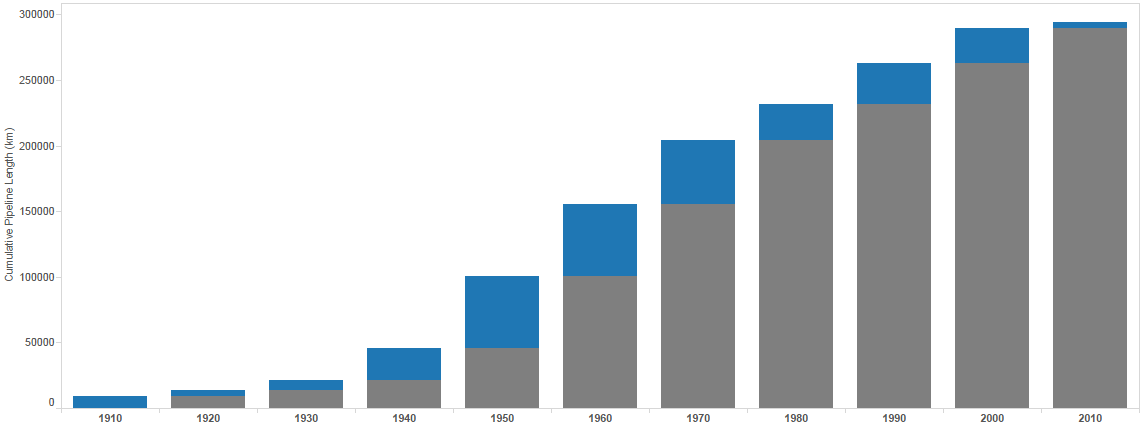
\includegraphics[keepaspectratio=true,scale=0.3]{../images/MileageHistogramCrop.png}
		\caption{Cumulative constructed pipeline kilometres by decade, from 1910 to 2010, stratified by new construction. 
			Blue is kilometres of new construction, and grey is cumulative existing kilometres.
		}
		\label{mileage-year}
	\end{figure}

	\begin{figure}
		\centering
		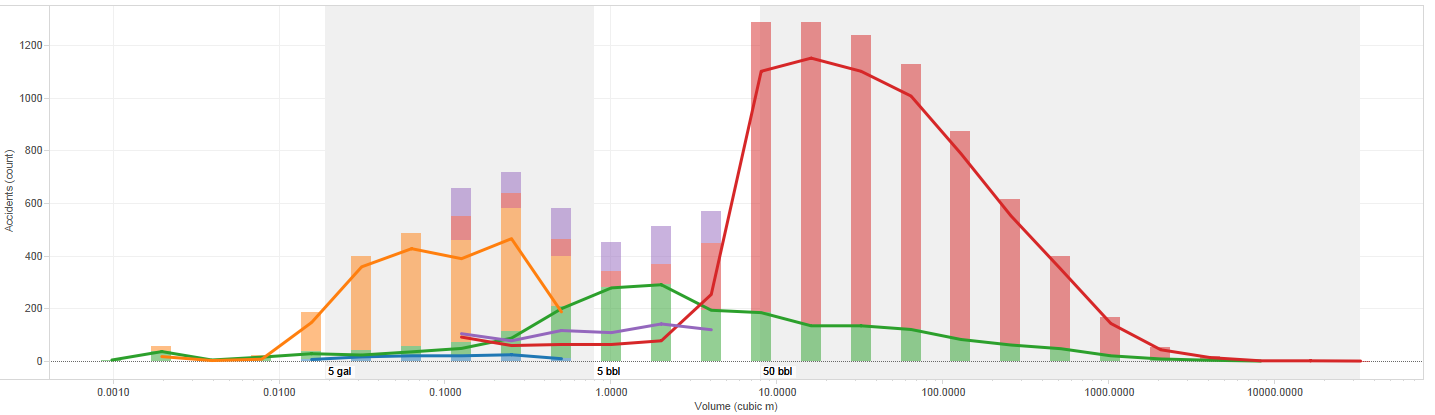
\includegraphics[keepaspectratio=true,scale=0.239]{../images/VolumeHistogramCrop.png}
		\caption{Logarithmic histogram of pipeline accident spill volumes, with bin boundaries defined by powers of 2, from $2^{-15}\left(\text{m}^3\right)$ to $2^{15} \left(\text{m}^3\right)$, stratified by reporting regimen.
			Stacked bars are the total accident counts, and proportion by reporting regimen. 
			Lines are individual distributions by reporting regimen. 
			Purple is voluntary reports preceding 2002, red is mandatory reports preceding 2002, orange is voluntary reports following 2002, green is mandatory reports following 2002, and blue is minimum reports following 2002.
			Shaded areas are the volumes between 5 gal and 5 bbl, and the volumes greater than 50 bbl.
		}
		\label{volume-histogram}
	\end{figure}

	\begin{figure}
		\centering
		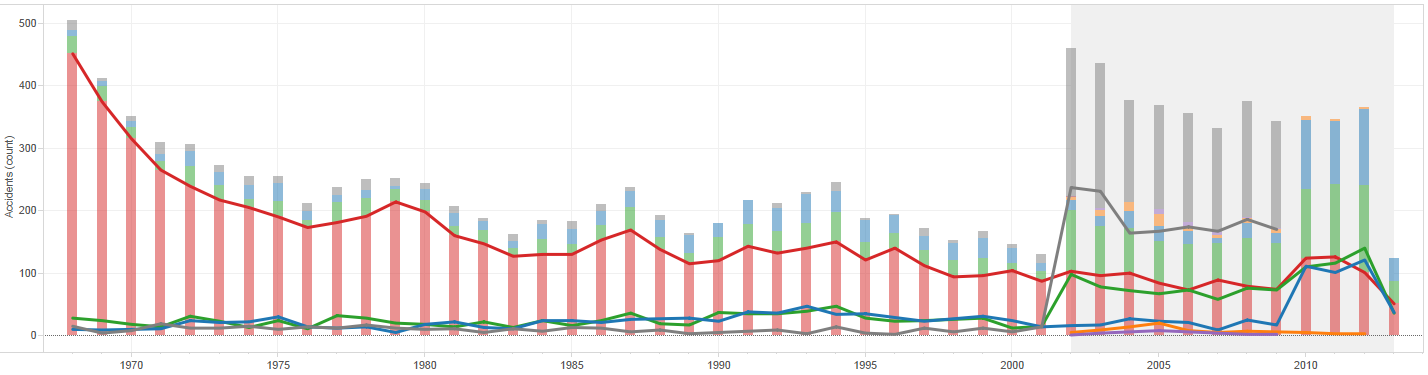
\includegraphics[keepaspectratio=true,scale=0.24]{../images/AccidentsYearCrop.png}
		\caption{Annual pipeline accident rate from 1968 to 2013, stratified by failure system. 
			Stacked bars are the total annual rates, and proportion by failure system. 
			Lines are individual rates by failure system. Red is main pipe body, green is mechanical components, blue is storage facilities, orange is support structures, purple is external fittings, and grey is not classified. 
			The years from 2002 onward are shaded.
		}\label{accidents-year}
	\end{figure}

	\begin{figure}
		\centering
		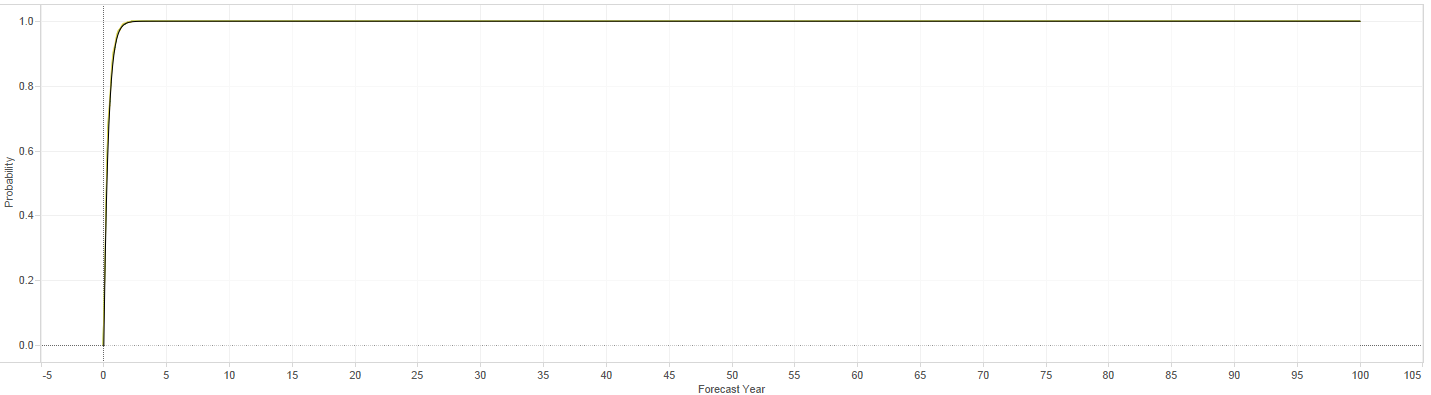
\includegraphics[keepaspectratio=true,scale=0.20]{../images/Forecast00000Crop.png}
		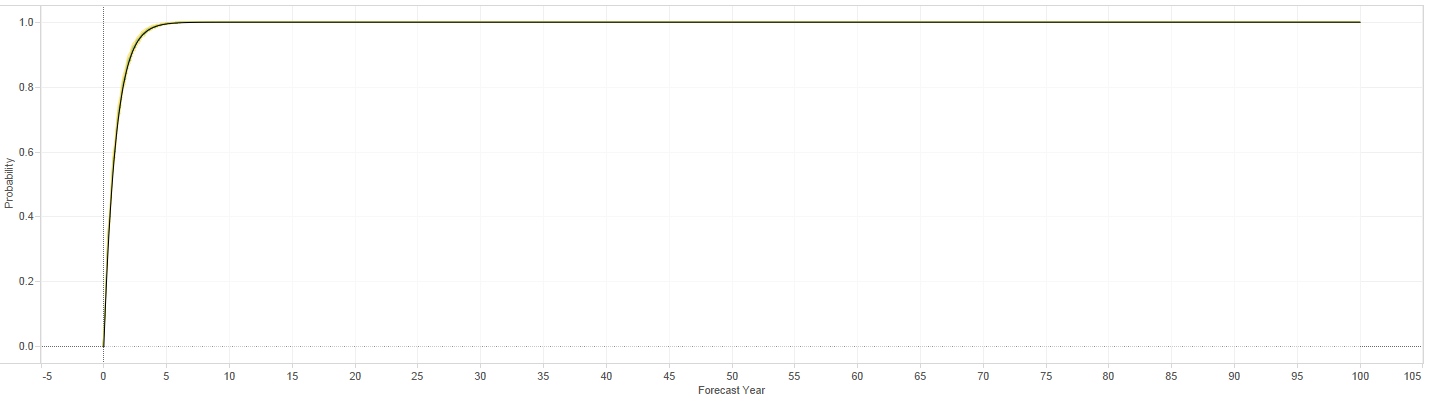
\includegraphics[keepaspectratio=true,scale=0.20]{../images/Forecast00001Crop.png}
		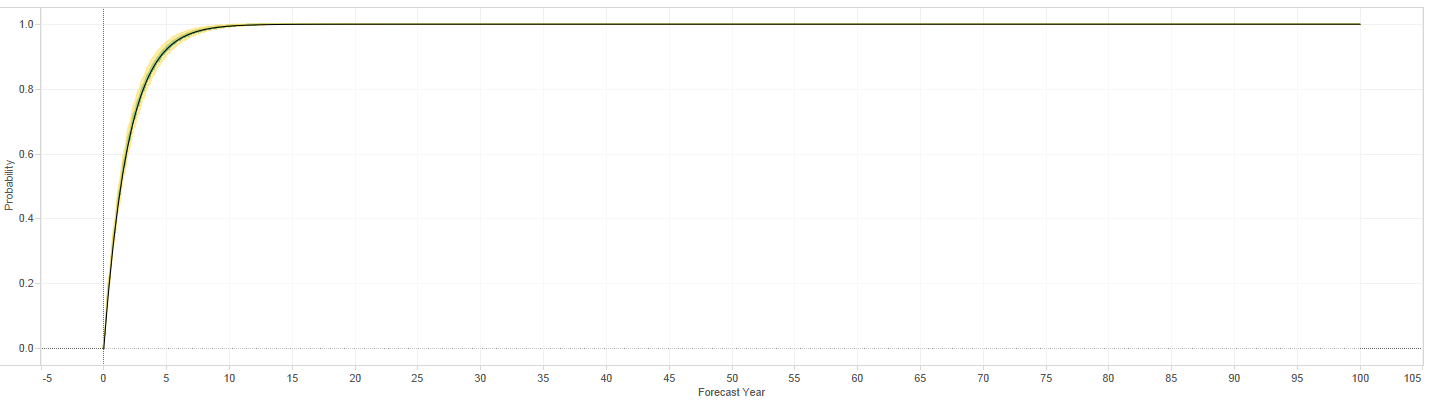
\includegraphics[keepaspectratio=true,scale=0.20]{../images/Forecast00010Crop.png}
		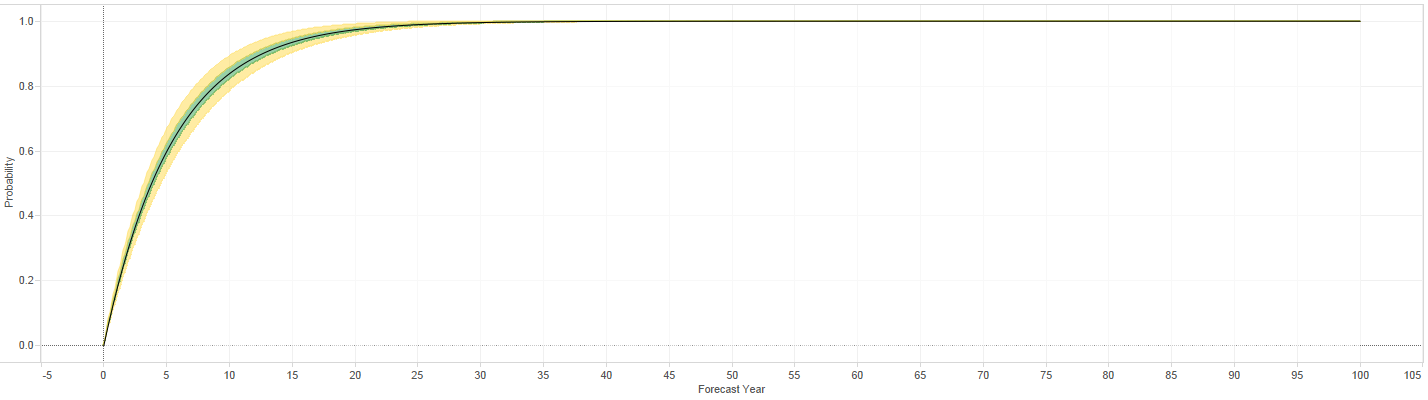
\includegraphics[keepaspectratio=true,scale=0.20]{../images/Forecast00100Crop.png}
		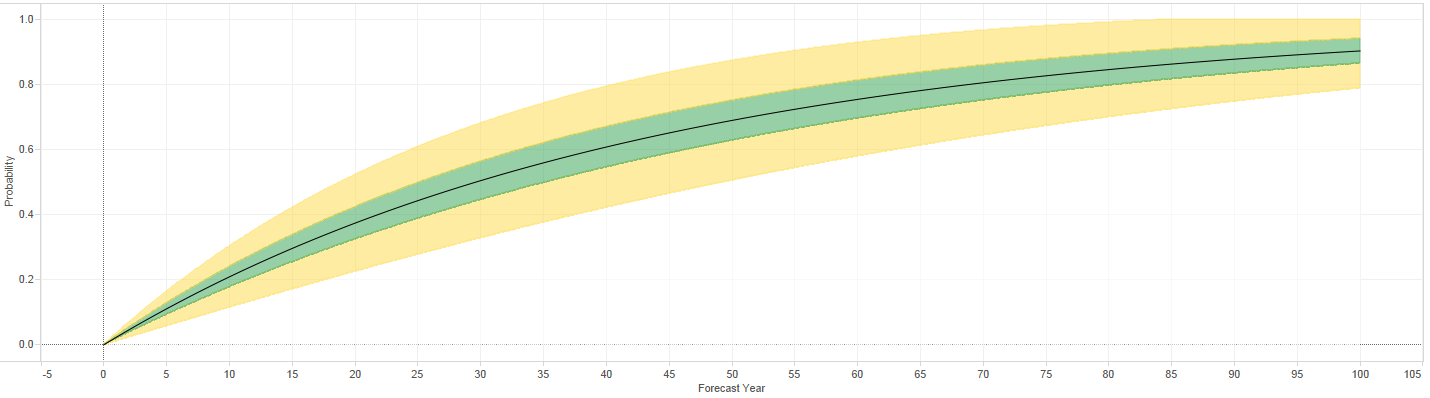
\includegraphics[keepaspectratio=true,scale=0.20]{../images/Forecast01000Crop.png}
		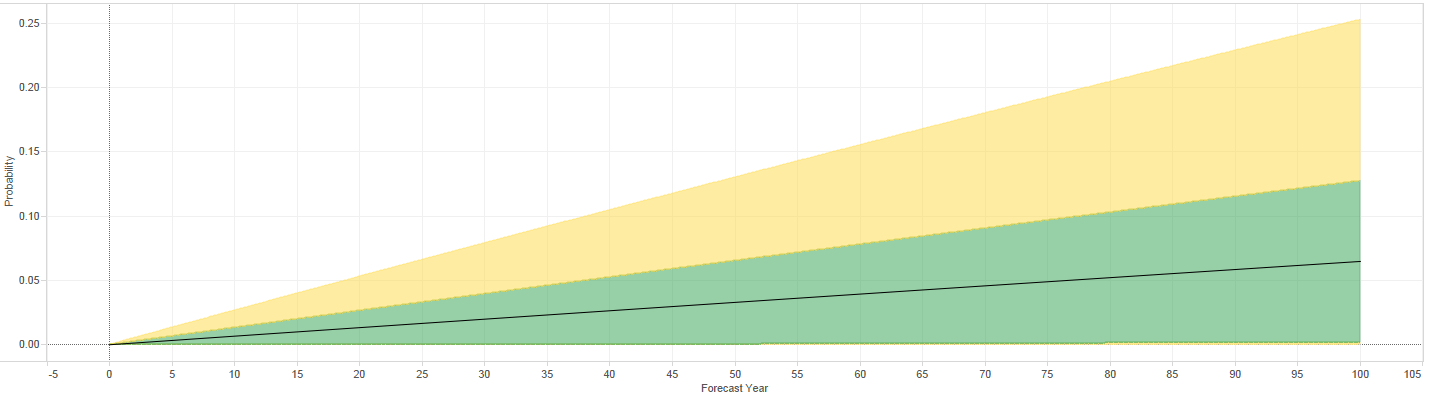
\includegraphics[keepaspectratio=true,scale=0.20]{../images/Forecast10000Crop.png}
		\caption{Forecast of the probability of at least 1 future pipeline accident out to 100 years, for 2340 km of pipeline.
			From top to bottom that plots are for a spill of at least 1, 10, 100, 1000, 10000 $\left(\text{m}^3\right)$.
			Green is 1 standard error confidence interval ($\approx$68.3\%), and yellow is 3 standard error confidence intervals ($\approx$99.7\%).
		}\label{forecast-estimate}
	\end{figure}

	\section{Discussion}\label{discussion}
	The theoretical consistency, and asymptotic efficiency of maximum likelihood estimators, and their continuous functions, as well as the calculation of the asymptotic variance from the Fisher information matrix, has been well established in the mathematical statistics literature since the mid 1950s.
	Yet it has only been within the last decade that sufficient desktop computational power has been widely available to make the use of these statistical theories implicitly common place.
	
	Mathematically, the confidence intervals represent true confidences in the forecast.
	Specifically, the canonical definition of the confidence interval is: if we assume the observed maximum likelihood estimators accurately reflect the actual values they are estimating, then the respective confidence intervals, $\approx$68.3\%, and $\approx$99.7\%, are the ranges in which we expect, $\approx$68.3\%, and $\approx$99.7\%, of the future observations to coincide. 
	The interpretation of the confidence intervals and levels is perhaps the most contentious part of this analysis.
	The debate on the interpretation of confidence intervals is part of a broader dialectic between the frequentest interpretation of statistical estimators, and the Bayesian interpretation of statistical estimators.

	An easier to resolve, but no less important, source of contention are three criticism of this analysis:
	first, that the selected data range was biased against pipeline development;
	second, that the variables selected as proxy measures for exposure were biased against pipeline development;
	third, that the assumptions over simplified the dynamics of pipeline accidents, so as to be biased against pipeline development.
	In all three cases we can clearly argue that results of this analysis are biased towards a favourable view of pipeline development; and further that any changes to the analysis would result in stronger evidence against pipeline development.
	
	With regard to the selection of data, that was used to forecast the probabilities of future pipeline accidents, as was specified in section \ref{application} only data on or after the year 2002 was used for in calculating the forecast.
	As figure \ref{accidents-year} illustrates this is well after annual accident rates had decreased to a steady state, particularly for accidents occurring in the main pipeline body.
	The 2012 rate of accidents occurring the main body of the pipeline is 4.5 times below the historical maximum of 451 pipeline body accidents observed in 1968.
	Furthermore, section \ref{application} illustrates how the increase in the number of accidents reported without a failure system corresponded with the change in reporting requirements after 2002; where all accidents with a volume over 5 bbl to be reported.
	Thus any selection of data that includes more of the historical data would bias the forecast towards predicting more frequent and larger accidents.

	With regard to using the decade of pipeline construction to calculate a proxy for the product of pipeline length and service usage time, the product is used in the denominator, so that over estimation of the product will underestimate the forecast probability.
	Clearly using the decade of pipeline construction will overestimate the total product; when compared to actual service usage time, and the affects of pipelines being decommissioning.
	Thus if we were to incorporate actual service usage time, including the decommissioning of pipelines, we would bias the forecast towards predicting more frequent accidents.

	With regard to the assumptions of the analysis being biased, through simplification, against pipeline development, the introduction of further orders of dependence in the variables would incorporate effects that would forecast more frequent pipeline accidents.
	If we were to consider higher order statistical correlations, that is that the events are no longer independent, then the only reasonable model is that of re-failure of previous accident sites.
	If we were to consider higher order dependence on forecast time, the only reasonable model would be of increasing material fatigue over time.
	Thus incorporation of any of these high order dependencies would bias the forecast towards predicting more frequent accidents.

	States share jurisdiction over safety and environmental enforcement with the \textit{US} federal government, leading to a regulatory heterogeneity under which pipelines operate.
	Furthermore, as evidenced by the voluntary reports, there is a heterogeneity in the environmental, and safety practices between pipeline operators.
	The difference between pipeline operators could be many fold, ranging from engineer differences, to bureaucratic differences, to differing priorities.

	The next stage of research should address the three major co-variates of the historical accident rate: the exponential dependence on the historical time, the dependence on the state in which the accident occurred, and the dependence on the operator of the pipeline in which the accident occurred.
	The statistically significant co-variates can be found through dimensional refinement, by the sequential application likelihood ratio test.

	While the data sets do consistently identify the states in which historical accidents have occurred, the identification of pipeline operators has not been as consistent.
	Part of the inconsistency is due to poor data entry in free text fields, but equally important has been the significant degree of economic dynamism in the pipeline industry
	The economic turn over has resulted in multiple re-namings, and changes of ownership in pipeline operators, effectively negating the unique numerical identifiers assigned by the \textit{PHMSA} to the pipeline operators.
	Table \ref{operator-degeneracy} summarizes the number of different operator names, and operator identifiers found in the mileage and accident data sets.
	\begin{longtable}{lrr}
		\caption{Tabulation of distinct operator identifiers, and names, by data source.}\label{operator-degeneracy}\\
		& \multicolumn{1}{l}{Mileage Reports} & \multicolumn{1}{l}{Accidents Reports}\\
		\hline
		\endfirsthead
		\caption{Continued from previous page.}\\
		& \multicolumn{1}{l}{Mileage Reports} & \multicolumn{1}{l}{Accident Reports}\\
		\hline
		\endhead
		\caption*{Continued on next page}
		\endfoot
		\endlastfoot
		Identifiers & 578 & 375\\
		Names & 950 & 371
	\end{longtable}
	The lengthy amount of manual cleaning, and industrial ownership research, necessary to have a consistent co-variate for the pipeline operators constrained the ambitions of this paper.
	As such we have left the statistical plan of the previous paragraph as a direction for future research.

	Further analysis and information are available on the website foreshortenedperspective.wordpress.com, including processed data sets.
	\appendix
	\section{Matrix Inversion}
	These appendices contain a collection of notes on the derivation of the estimators, and their variances.
	For the most part, these sections were written for the benefit of the author; to collate the derivations used in writing this letter.

	We begin with the derivation of a formula for the inverse matrix of the family of matrices to which the Fisher information matrix of parameter estimators belongs.
	The setup is a bit cumbersome, but the final result is a simple closed form for the inverse matrix.

	Among many objects, we can form $3$ particular matrices from an orthonormal basis $\hat{e}_1, \dots , \hat{e}_{k-1}$ of a $k-1$ dimensional vector space.
	First, we have the identity matrix
	\begin{IEEEeqnarray*}{rCl}
		I & = & \sum_{i=1}^{k-1} \hat{e}_i\hat{e}_i^\dagger
	\end{IEEEeqnarray*}
	Next, for each vector $\vec{a}$ we have the diagonal matrix
	\begin{IEEEeqnarray*}{rCl}
		diag\left(\vec{a} \right) & = & \sum_{i=1}^{k-1} \hat{e}_i \left(\vec{a}^\dagger \hat{e}_i\right) \hat{e}_i^\dagger
	\end{IEEEeqnarray*}
	Finally, the projection matrix 
	\begin{IEEEeqnarray*}{rCl}
		P & = & \hat{1}\hat{1}^\dagger 
	\end{IEEEeqnarray*}
	where we have the vectors 
	\begin{IEEEeqnarray*}{rCl}
		\hat{1} & = & \frac{1}{\sqrt{k-1}} \sum_{i=1}^{k-1} \hat{e}_i 
	\end{IEEEeqnarray*}
	These matrices, and vectors, obey a number of useful identities. 

	The set of matrices formed by $diag\left(\vec{a}\right)$ is a ring, that is it is closed under element wise addition and multiplication.
	In particular if $0 \neq \vec{a}^\dagger \hat{e}_i$ for all $i$ then 
	\begin{IEEEeqnarray*}{rCl}
		diag\left( \vec{a} \right)^{-1} & = & diag\left( \vec{a^{-1}} \right)
	\end{IEEEeqnarray*}
	where 
	\begin{IEEEeqnarray*}{rCl}
		\vec{a^{-1}} & = & \sum_{i=1}^n \left(\vec{a}^\dagger \hat{e}_i\right)^{-1} \hat{e}_i
	\end{IEEEeqnarray*}
	The vector $\vec{1}$ recovers the vector $\vec{a}$ from $diag\left( \vec{a} \right)$, through $diag\left( \vec{a} \right) \vec{1} = \vec{a}$.
	This implies that product of the project matrix $P$ and the diagonal matrix $diag\left( \vec{a} \right)$ results in the matrix 
	\begin{IEEEeqnarray*}{rCl}
		P diag\left( \vec{a} \right) & = & \frac{1}{k-1} \vec{1} \vec{a}^\dagger
	\end{IEEEeqnarray*}
	Furthermore, the double product of the project matrix $P$ and the diagonal matrix $diag\left( \vec{a} \right)$ results in the idempotent 
	\begin{IEEEeqnarray*}{rCl}
		P diag\left( \vec{a} \right) P diag\left( \vec{a} \right) & = & \frac{\vec{1}^\dagger \vec{a}}{k-1}  P diag\left( \vec{a} \right)
	\end{IEEEeqnarray*}

	The Fisher information matrix of the estimators of the parameters is of the general form $A = diag\left( \vec{a} \right) + \alpha P$, for some scalar constant $\alpha$, and vector $\vec{a}$ such that $0 \neq \vec{a}^\dagger \hat{e}_i$ for all $i$.
	After exploring the matrix Taylor series expansion for the inverse, we strike upon a trial solution of the form
	\begin{IEEEeqnarray*}{rCl}
		A^{-1} & = & diag\left( \vec{a^{-1}} \right) + \beta diag\left( \vec{a^{-1}} \right) P diag\left( \vec{a^{-1}} \right)
	\end{IEEEeqnarray*}
	for some scalar constant $\beta$, that needs to be determined.
	Requiring that $A^{-1}A = I$ we then have
	\begin{IEEEeqnarray*}{rCl}
		I
			& = & A^{-1}A\\
			& = & I + \left(\frac{\alpha}{k-1} + \frac{\beta}{k-1} + \frac{\alpha \beta \vec{1}^\dagger \vec{a^{-1}}}{\left(k-1\right)^2}\right) \vec{a^{-1}}\vec{1}^\dagger 
	\end{IEEEeqnarray*}
	Which yields the value for $\beta$ of 
	\begin{IEEEeqnarray*}{rCl}
		\beta & = & -\frac{\alpha \left(k-1\right)}{\left(k-1\right) + \alpha \vec{1}^\dagger \vec{a^{-1}}}
	\end{IEEEeqnarray*}
	and thus the inverse is 
	\begin{IEEEeqnarray*}{rCl}
		A^{-1} & = & diag\left( \vec{a^{-1}} \right) -\frac{\alpha \left(k-1\right)}{\left(k-1\right) + \alpha \vec{1^\dagger} \vec{a^{-1}}} diag\left( \vec{a^{-1}} \right) P diag\left( \vec{a^{-1}} \right)
	\end{IEEEeqnarray*}

	\section{Parameter Estimation}
	With this machinery in place we continue with deriving the estimators for the parameters of the joint probability distribution, assuming an observed pipeline length of $l$, service usage time $t$, and accident size bins $0 = b_0 < b_1 < \cdots < b_{k-1} < b_k = \infty$.
	\begin{IEEEeqnarray*}{rCl}
		\IEEEeqnarraymulticol{3}{l}{\mathbb{P}\left[N_1^{\left(lt\right)} = n_1, \dots , N_k^{\left(lt\right)} = n_k \right]} \\
			\qquad & = & \frac{\left( l t \lambda \right)^{n_{1:k}}}{n_{1:k}!} e^{- l t \lambda} \binom{n_{1:k}}{n_1 \cdots n_k}\rho_1^{n_1} \cdots \left(1 - \rho_{1:k-1} \right)^{n_k}
	\end{IEEEeqnarray*}
	Following in the usual method we begin with the log-likelihood function in the parameters $\lambda$ and $\rho_i$.
	\begin{IEEEeqnarray*}{rCl}
		\Lambda^{\left(lt\right)} & = & \ln\left( \mathbb{P}\left[ N_1^{\left(lt\right)} = n_1, \dots , N_k^{\left(lt\right)} = n_k \right]\right) \\
			& = & \ln\left( \frac{\left( l t \right)^{n_{1:k}}}{n_{1:k}!} \binom{n_{1:k}}{n_1 \cdots n_k} \right) + n_{1:k} \ln\left( \lambda \right) -  l t \lambda\\
			&   & \quad + n_1 \ln\left( \rho_1 \right) + \cdots + n_k \ln\left(1 - \rho_{1:k-1}\right)
	\end{IEEEeqnarray*}
	The first and second order partial derivatives are
	\begin{IEEEeqnarray*}{rCl}
		\frac{\partial \Lambda^{\left(lt\right)}}{\partial \lambda} & = & \frac{n_{1:k}}{\lambda} - l t\\
		\frac{\partial \Lambda^{\left(lt\right)}}{\partial \rho_i} & = & \frac{n_i}{\rho_i} - \frac{n_k}{1 - \rho_{1:k-1}}\\
		\frac{\partial^2 \Lambda^{\left(lt\right)}}{\partial \lambda^2} & = & - \frac{n_{1:k}}{\lambda^2}\\
		\frac{\partial^2 \Lambda^{\left(lt\right)}}{\partial \lambda \partial \rho_i} & = & 0\\
		\frac{\partial^2 \Lambda^{\left(lt\right)}}{\partial \rho_i^2} & = & - \frac{n_i}{\rho_i^2} - \frac{n_k}{\left(1 - \rho_{1:k-1}\right)^2}\\
		\frac{\partial^2 \Lambda^{\left(lt\right)}}{\partial \rho_i \partial \rho_j} & = & - \frac{n_k}{\left(1 - \rho_{1:k-1}\right)^2}
	\end{IEEEeqnarray*}
	Equating the first partial derivatives to $0$ yields the maximum likelihood estimators
	\begin{IEEEeqnarray*}{rCl}
		\hat{\lambda} & = & \frac{N_{1:k}^{\left(lt\right)}}{l t}\\
		\hat{\rho}_j & = & \frac{N_j^{\left(lt\right)}}{N_{1:k}^{\left(lt\right)}}
	\end{IEEEeqnarray*}
	The estimators are the usual unbiased estimators from the standard statistics curriculum
	\begin{IEEEeqnarray*}{rCl}
		\mathbb{E} \left[ \hat{\lambda} \right]
			& = & \frac{1}{l t} \mathbb{E} \left[ N_{1:k}^{\left(lt\right)} \right]\\
			& = & \lambda\\
		\mathbb{E} \left[ \hat{\rho}_j \right]
			& = & \mathbb{E} \left[ \mathbb{E} \left[\left. \hat{\rho}_j \right\| N_{1:k}^{\left(lt\right)} \right] \right]\\
			& = & \mathbb{E} \left[ \frac{1}{N_{1:k}^{\left(lt\right)}} \mathbb{E} \left[ \left. N_j^{\left(lt\right)} \right\| N_{1:k}^{\left(lt\right)} \right] \right]\\
			& = & \mathbb{E} \left[ \frac{1}{N_{1:k}^{\left(lt\right)}} N_{1:k}^{\left(lt\right)} \rho_j \right]\\
			& = & \rho_j
	\end{IEEEeqnarray*}
	The Fisher information matrix is expectation of the matrix of second order partial derivatives 
	\begin{IEEEeqnarray*}{rCl}
		- \mathbb{E} \left[ \partial^2 \Lambda^{\left(lt\right)} \right] & = & \mathbb{E}
		\begin{bmatrix}
			\frac{N_{1:k}^{\left(lt\right)}}{\lambda^2} & \ldots                                                                                                 & 0      & \ldots \\
			\vdots                                      & \frac{N_1^{\left(lt\right)}}{\rho_1^2} + \frac{N_k^{\left(lt\right)}}{\left(1 - \rho_{1:k-1}\right)^2} & \ldots & \frac{N_k^{\left(lt\right)}}{\left(1 - \rho_{1:k-1}\right)^2} \\
			0                                           & \vdots                                                                                                 & \ddots & \vdots \\
			\vdots                                      & \frac{N_k^{\left(lt\right)}}{\left(1 - \rho_{1:k-1}\right)^2}                                          & \ldots & \frac{N_{k-1}^{\left(lt\right)}}{\rho_{k-1}^2} + \frac{N_k^{\left(lt\right)}}{\left(1 - \rho_{1:k-1}\right)^2}
		\end{bmatrix}\\
		& = &
		\begin{bmatrix}
			\frac{lt}{\lambda} & \ldots                                                         & 0      & \ldots \\
			\vdots             & \frac{lt \lambda}{\rho_1} + \frac{lt \lambda}{1 - \rho_{1:k-1}} & \ldots & \frac{lt \lambda}{1 - \rho_{1:k-1}} \\
			0                  & \vdots                                                         & \ddots & \vdots \\
			\vdots             & \frac{lt \lambda}{1 - \rho_{1:k-1}}                            & \ldots & \frac{lt \lambda}{\rho_{k-1}} + \frac{lt \lambda}{1 - \rho_{1:k-1}}
		\end{bmatrix}
	\end{IEEEeqnarray*}
	In a first application of the matrix inversion formula derived at the begin of this section we find that the Cramer-Rao lower bound for the covariance of the simultaneous parameter estimates of $\hat{\lambda}$ and $\hat{\rho_j}$ is given by
	\begin{IEEEeqnarray*}{rCl}
		\mathbb{C}ov \left[\hat{\lambda}, \hat{\rho}_1, \dots , \hat{\rho}_{k-1} \right] & = &
		- \mathbb{E} \left[ \partial^2 \Lambda^{\left(lt\right)} \right]^{-1}\\
		& = &
		\begin{bmatrix}
			\frac{\lambda}{lt} & \ldots                                            & 0      & \ldots \\
			\vdots             & \frac{\rho_1 \left(1 - \rho_1\right)}{lt \lambda} & \ldots & - \frac{\rho_1 \rho_{k-1}}{lt \lambda} \\
			0                  & \vdots                                            & \ddots & \vdots \\
			\vdots             & - \frac{\rho_1 \rho_{k-1}}{lt \lambda}            & \ldots & \frac{\rho_{k-1} \left(1 - \rho_{k-1}\right)}{lt \lambda}
		\end{bmatrix}
	\end{IEEEeqnarray*}
	in which we can recognize the usual multinomial and Poisson covariance formulas found in the standard statistical curriculum.
	The covariance demonstrates the consistency of the estimators $\hat{\lambda}$ and $\hat{\rho_j}$; as the covariance vanishes in the limit of large product $lt$; which, in stochastic processes, acts in place of the usual large sample limit.

	\section{Forecast Estimation}
	We can make use of these results to estimate the probability of a spill of at least size $b_r$ within a fixed future time span of $\tilde{t}$, and a fixed future pipeline length of $\tilde{l}$.
	The probability of at least $1$ spill event of size at least $b_r$, given the parameters $\lambda$ and $\rho_i$, is the complement of the event of either no spills occurring, or all the spills are of a size less than $b_r$, thus we define the parameter function
	\begin{IEEEeqnarray*}{rCl}
		h\left(\lambda, \rho_j \right)
			& = & 1 - \mathbb{P}\left[N_{1:k}^{\left(\tilde{l} \tilde{t} \right)} = 0 \right] - \mathbb{P}\left[0 < N_{1:r}^{\left(\tilde{l} \tilde{t} \right)} = N_{1:k}^{\left(\tilde{l} \tilde{t} \right)} \right]\\
			& = & 1 - e^{- \tilde{l} \tilde{t} \lambda} - \mathbb{E}\left[\mathbb{P}\left[\left. N_{1:r}^{\left(\tilde{l} \tilde{t} \right)} = N_{1:k}^{\left(\tilde{l} \tilde{t} \right)} \right\| N_{1:k}^{\left(\tilde{l} \tilde{t} \right)} \right] \mathbb{I}\left[ 0 < N_{1:k}^{\left(\tilde{l} \tilde{t} \right)} \right] \right]\\
			& = & 1 - e^{- \tilde{l} \tilde{t} \lambda} - \sum_{n=1}^\infty \frac{\left( \tilde{l} \tilde{t} \lambda \rho_{1:r} \right)^n}{n!} e^{- \tilde{l} \tilde{t} \lambda} \\
			& = & 1 - e^{- \tilde{l} \tilde{t} \lambda \left(1 - \rho_{1:r} \right)}
	\end{IEEEeqnarray*}
	Because $h\left(\lambda, \rho_j \right)$ is a continuous function of the parameters $\lambda$ and $\rho_i$, it follows, by the consistent of the maximum likelihood estimators $\hat{\lambda}$ and $\hat{\rho}_j$, that
	\begin{IEEEeqnarray*}{rCl}
		H_r^{\left(\tilde{l} \tilde{t} \right)}
			& = & h\left(\hat{\lambda}, \hat{\rho}_j \right)\\
			& = & 1 - \exp{\left(- \frac{\tilde{l} \tilde{t}}{lt} N_{r+1:k}^{\left(lt\right)} \right)}
	\end{IEEEeqnarray*} 
	 is the maximum likelihood estimator of $h\left(\lambda, \rho_j \right)$, and thus a consistent estimator. 
	
	By the asymptotic relative efficiency of the maximum likelihood estimators, we have that the asymptotic variance of $H_r^{\left(\tilde{l} \tilde{t} \right)}$ is given by
	\begin{IEEEeqnarray*}{rCl}
		\mathbb{V}ar\left[H_r^{\left(\tilde{l} \tilde{t} \right)}\right]
			& = & \left(\left. \partial h \right|_{\lambda = \hat{\lambda}, \rho_j = \hat{\rho}_j} \right)^\dagger \left(\left. - \partial^2 \Lambda \right|_{\lambda = \hat{\lambda}, \rho_j = \hat{\rho}_j}\right)^{-1} \left(\left. \partial h \right|_{\lambda = \hat{\lambda}, \rho_j = \hat{\rho}_j}\right)
	\end{IEEEeqnarray*}
	The vector of first order partial derivatives is given by
	\begin{IEEEeqnarray*}{rCl}
		\left. \partial h \right|_{\lambda = \hat{\lambda}, \rho_j = \hat{\rho}_j} & = & 
		\tilde{l} \tilde{t} e^{- \tilde{l} \tilde{t} \hat{\lambda} \left(1 - \hat{\rho}_{1:r} \right) }
		\begin{bmatrix}
			\left(1 - \hat{\rho}_{1:r}\right)\\
			- \hat{\lambda}\\
			\vdots\\
			- \hat{\lambda}\\
			0\\
			\vdots
		\end{bmatrix}
	\end{IEEEeqnarray*}
	where the last $k - r - 1$ elements are zero.
	The asymptotic estimator of the Fisher information matrix is given by
	\begin{IEEEeqnarray*}{rCl}
		\left. - \partial^2 \Lambda^{\left(lt\right)} \right|_{\lambda = \hat{\lambda}, \rho_j = \hat{\rho}_j} & = & 
		\begin{bmatrix}
			\frac{lt}{\hat{\lambda}} & \ldots                                                                                  & 0      & \ldots \\
			\vdots                   & \frac{lt \hat{\lambda}}{\hat{\rho}_1} + \frac{lt \hat{\lambda}}{1 - \hat{\rho}_{1:k-1}} & \ldots & \frac{lt \hat{\lambda}}{1 - \hat{\rho}_{1:k-1}} \\
			0                        & \vdots                                                                                  & \ddots & \vdots \\
			\vdots                   & \frac{lt \hat{\lambda}}{1 - \hat{\rho}_{1:k-1}}                                         & \ldots & \frac{lt \hat{\lambda}}{\hat{\rho}_{k-1}} + \frac{lt \hat{\lambda}}{1 - \hat{\rho}_{1:k-1}}
		\end{bmatrix}
	\end{IEEEeqnarray*}
	Applying the matrix inversion formula with vector $\vec{a}$, and scalar $\alpha$
	\begin{IEEEeqnarray*}{rCl}
		\vec{a} & = &
		\begin{bmatrix}
			\frac{1}{\hat{\rho}_1}\\
			\vdots\\
			\frac{1}{\hat{\rho}_{k-1}}
		\end{bmatrix}\\
		\alpha & = & \frac{k-1}{1 - \hat{\rho}_{1:k-1}}
	\end{IEEEeqnarray*}
	results in the inverse, that exactly replicates the covariance found earlier
	\begin{IEEEeqnarray*}{rCl}
		\left( \left. - \partial^2 \Lambda \right|_{\lambda = \hat{\lambda}, \rho_j = \hat{\rho}_j} \right)^{-1} & = & 
		\begin{bmatrix}
			\frac{\hat{\lambda}}{lt} & \ldots                                                        & 0      & \ldots \\
			\vdots             & \frac{\hat{\rho}_1 \left(1 - \hat{\rho}_1\right)}{lt \hat{\lambda}} & \ldots & - \frac{\hat{\rho}_1 \hat{\rho}_{k-1}}{lt \hat{\lambda}} \\
			0                  & \vdots                                                              & \ddots & \vdots \\
			\vdots             & - \frac{\hat{\rho}_1 \hat{\rho}_{k-1}}{lt \hat{\lambda}}            & \ldots & \frac{\hat{\rho}_{k-1} \left(1 - \hat{\rho}_{k-1}\right)}{lt \hat{\lambda}}
		\end{bmatrix}
	\end{IEEEeqnarray*}
	Taking the final matrix product yields the asymptotic variance estimator
	\begin{IEEEeqnarray*}{rCl}
		\mathbb{V}ar\left[H_r^{\left(\tilde{l} \tilde{t} \right)}\right]
			& = & \frac{\hat{\lambda}}{lt} \left(1 - \hat{\rho}_{1:r} \right) \left(\tilde{l} \tilde{t} \right)^2 \exp\left(-2 \tilde{l}\tilde{t} \hat{\lambda} \left(1 - \hat{\rho}_{1:r}\right)\right)
	\end{IEEEeqnarray*}
	It follows from the asymptotic relative efficiency of maximum likelihood estimators that the statistic
	\begin{IEEEeqnarray*}{rCl}
		Z & = & \frac{H_r^{\left(\tilde{l} \tilde{t} \right)} - h\left(\lambda, \rho_j \right)}{\sqrt{\mathbb{V}ar\left[H_r^{\left(\tilde{l} \tilde{t} \right)}\right]}}
	\end{IEEEeqnarray*}
	is asymptotically standard normal distributed, thus allowing for the calculation of confidence intervals for the future probability of an accident $h\left(\lambda, \rho_j \right)$.

	This result can be generalized to arbitrary accident size set $B$ that are Borel measurable subsets $B \subseteq \mathbb{R}^{+}$ of the positive real line; by combining the arbitrary choice of bins with the fact that the $\sigma$-algebra of intervals generates the Borel measurable sets.

	\section{Classification of Accidents}

	\begin{figure}
		\centering
		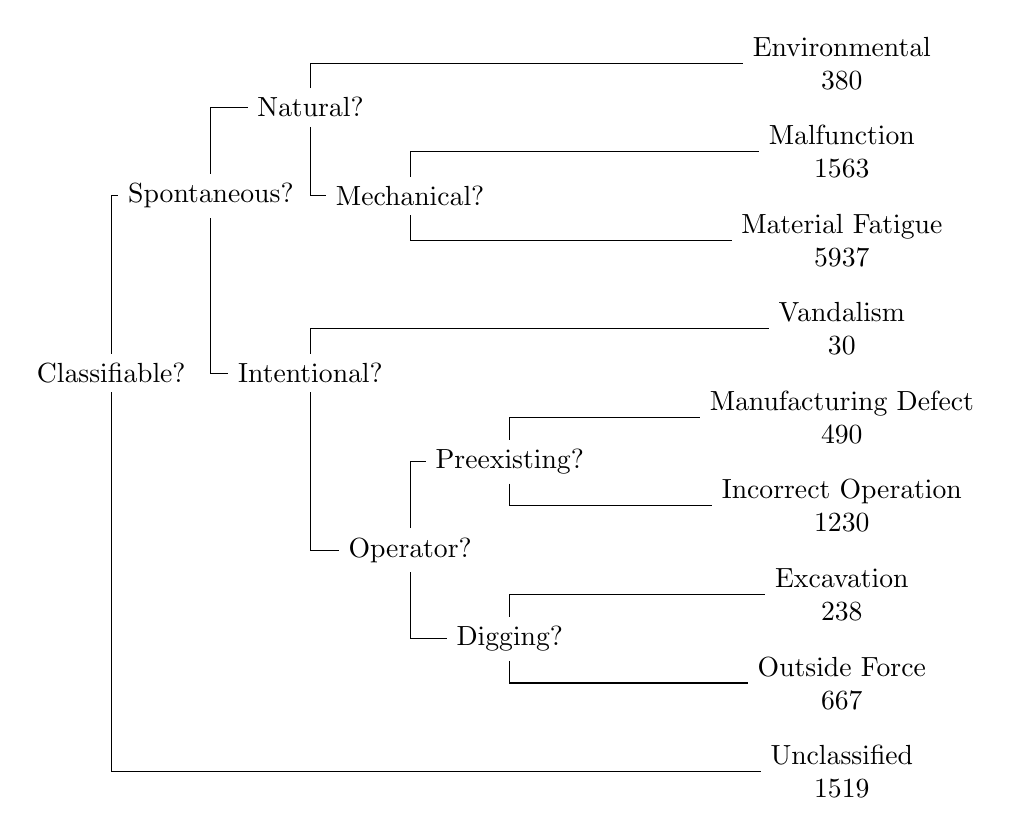
\begin{tikzpicture} [grow'=right,edge from parent path={(\tikzparentnode) |- (\tikzchildnode)},every node/.style={align=center}]
			\node {Classifiable?}
				child [sibling distance=128pt,level distance=36pt]
				{
					node {Spontaneous?} 
					child [sibling distance=64pt]
					{
						node {Natural?}
						child [sibling distance=32pt,level distance=192pt]
						{
							node {Environmental\\380}
						}
						child
						{
							node {Mechanical?}
							child [sibling distance=32pt,level distance=156pt]
							{
								node {Malfunction\\1563}
							}
							child [sibling distance=32pt,level distance=156pt]
							{
								node {Material Fatigue\\5937}
							}
						}
					}
					child [sibling distance=128pt]
					{
						node {Intentional?}
						child [sibling distance=32pt,level distance=192pt]
						{
							node {Vandalism\\30}
						}
						child
						{
							node {Operator?}
							child [sibling distance=64pt]
							{
								node {Preexisting?}
								child [sibling distance=32pt,level distance=120pt]
								{
									node {Manufacturing Defect\\490}
								}
								child [sibling distance=32pt,level distance=120pt]
								{
									node {Incorrect Operation\\1230}
								}
							}
							child [sibling distance=64pt]
							{
								node {Digging?}
								child [sibling distance=32pt,level distance=120pt]
								{
									node {Excavation\\238}
								}
								child [sibling distance=32pt,level distance=120pt]
								{
									node {Outside Force\\667}
								}
							}
						}
					}
				}
				child [sibling distance=288pt,level distance=264pt]
				{
					node {Unclassified\\1519}
				};
		\end{tikzpicture}
		\caption{Decision tree rubric to classify accident causes. Yes decisions travel upward, no decisions downward. 
			Accident counts are below each leaf node.
		}
		\label{cause-decision}
	\end{figure}

	\begin{figure}
		\centering
		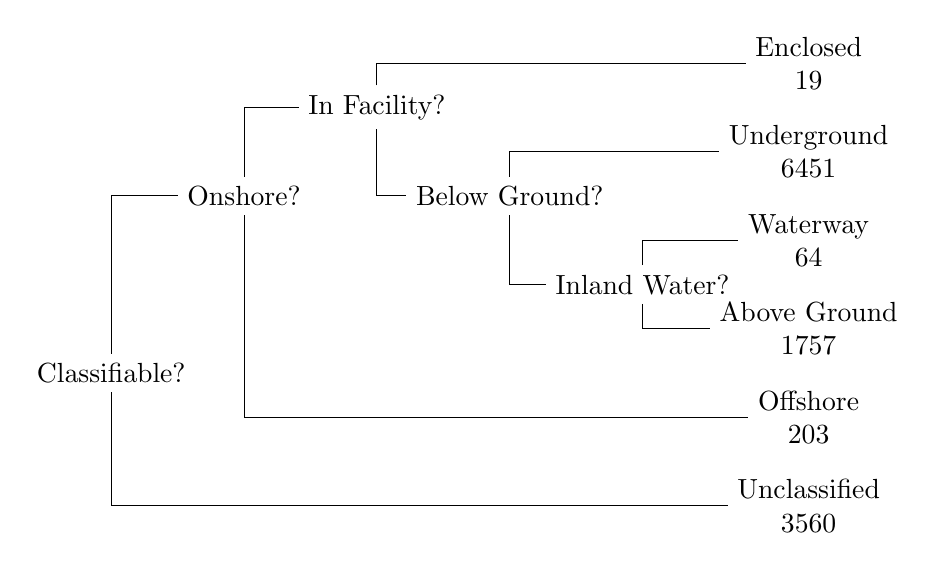
\begin{tikzpicture} [grow'=right,edge from parent path={(\tikzparentnode) |- (\tikzchildnode)},every node/.style={align=center}]
			\node {Classifiable?}
				child [sibling distance=128pt,level distance=48pt]
				{
					node {Onshore?}
					child [sibling distance=64pt]
					{
						node {In Facility?}
						child [sibling distance=32pt,level distance=156pt]
						{
							node {Enclosed\\19}
						}
						child [sibling distance=64pt]
						{
							node {Below Ground?}
							child [sibling distance=32pt,level distance=108pt]
							{
								node {Underground\\6451}
							}
							child
							{
								node {Inland Water?}
								child [sibling distance=32pt,level distance=60pt]
								{
									node {Waterway\\64}
								}
								child [sibling distance=32pt,level distance=60pt]
								{
									node {Above Ground\\1757}
								}
							}
						}
					}
					child [sibling distance=160pt,level distance=204pt]
					{
						node {Offshore\\203}
					}
				}
				child [sibling distance=96pt,level distance=252pt]
				{
					node {Unclassified\\3560}
				};
		\end{tikzpicture}
		\caption{Decision tree rubric to classify accident location types. Yes decisions travel upward, no decisions downward. 
			Accident counts are below each leaf node.
		}
		\label{location-decision}
	\end{figure}

	\begin{figure}
		\centering
		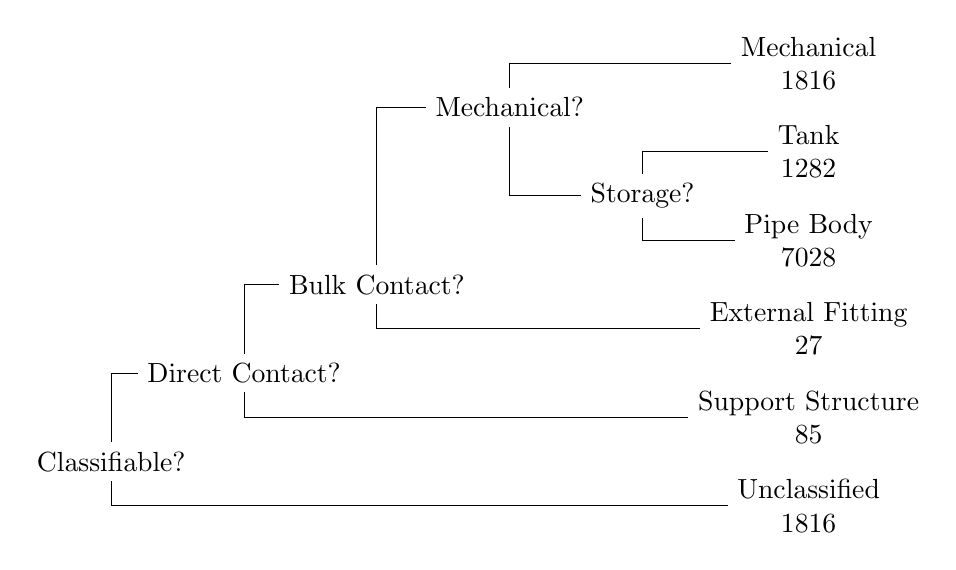
\begin{tikzpicture} [grow'=right,edge from parent path={(\tikzparentnode) |- (\tikzchildnode)},every node/.style={align=center}]
			\node {Classifiable?}
				child [sibling distance=64pt,level distance=48pt]
				{
					node {Direct Contact?}
					child [sibling distance=64pt]
					{
						node {Bulk Contact?}
						child [sibling distance=128pt]
						{
							node {Mechanical?}
							child [sibling distance=32pt,level distance=108pt]
							{
								node {Mechanical\\1816}
							}
							child [sibling distance=64pt]
							{
									node {Storage?}
									child [sibling distance=32pt,level distance=60pt]
									{
										node {Tank\\1282}
									}
									child[sibling distance=32pt,level distance=60pt]
									{
									node {Pipe Body\\7028}
								}
							}
						}
						child [sibling distance=32pt,level distance=156pt]
						{
							node {External Fitting\\27}
						}
					}
					child [sibling distance=32pt,level distance=204pt]
					{
						node {Support Structure\\85}
					}
				}
				child [sibling distance=32pt,level distance=252pt]
				{
					node {Unclassified\\1816}
				};
		\end{tikzpicture}
		\caption{Decision tree rubric to classify accident failure systems. Yes decisions travel upward, no decisions downward.
			Accident counts are below each leaf node.
		}
		\label{system-decision}
	\end{figure}

	\begin{figure}
		\centering
		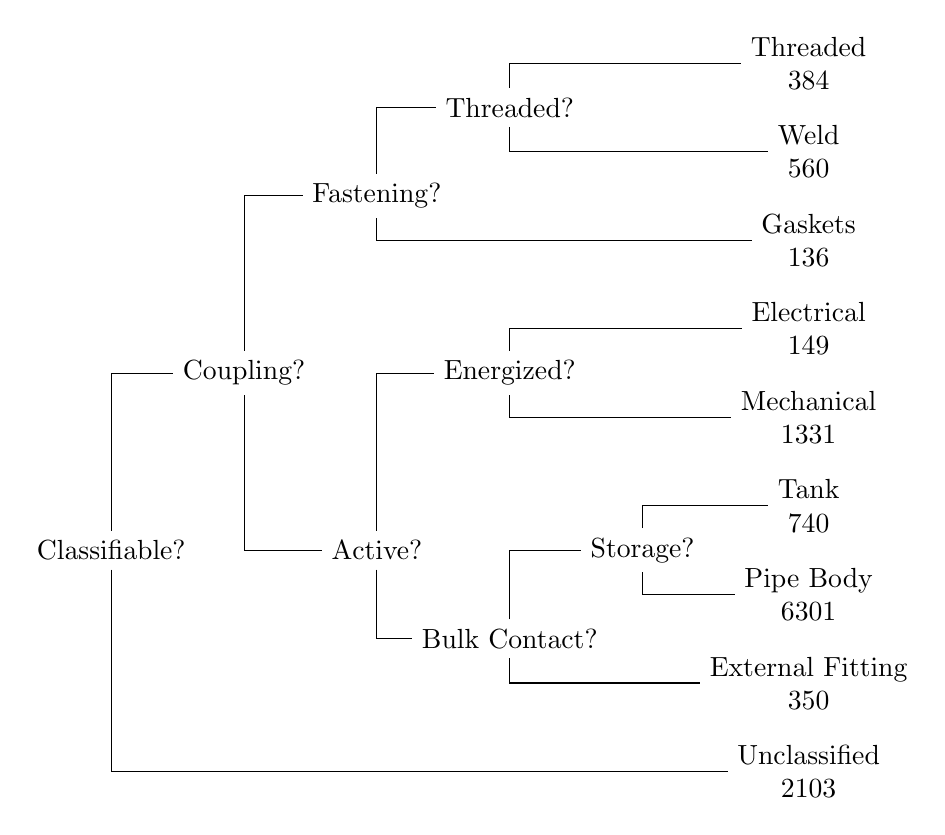
\begin{tikzpicture} [grow'=right,edge from parent path={(\tikzparentnode) |- (\tikzchildnode)},every node/.style={align=center}]
			\node {Classifiable?}
				child [sibling distance=128pt,level distance=48pt]
				{
					node {Coupling?}
					child
					{
						node {Fastening?}
						child [sibling distance=64pt]
						{
							node {Threaded?}
							child [sibling distance=32pt,level distance=108pt]
							{
								node {Threaded\\384}
							}
							child [sibling distance=32pt,level distance=108pt]
							{
								node {Weld\\560}
							}
						}
						child [sibling distance=32pt,level distance=156pt]
						{
							node {Gaskets\\136}
						}
					}
					child [sibling distance=128pt]
					{
						node {Active?}
						child
						{
							node {Energized?}
							child [sibling distance=32pt,level distance=108pt]
							{
								node {Electrical\\149}
							}
							child [sibling distance=32pt,level distance=108pt]
							{
								node {Mechanical\\1331}
							}
						}
						child [sibling distance=64pt]
						{
							node {Bulk Contact?}
							child
							{
								node {Storage?}
								child [sibling distance=32pt,level distance=60pt]
								{
									node {Tank\\740}
								}
								child [sibling distance=32pt,level distance=60pt]
								{
									node {Pipe Body\\6301}
								}
							}
							child [sibling distance=32pt,level distance=108pt]
							{
								node {External Fitting\\350}
							}
						}
					}
				}
				child [sibling distance=160pt,level distance=252pt]
				{
					node {Unclassified\\2103}
				};
		\end{tikzpicture}
		\caption{Decision tree rubric to classify accident failure parts. Yes decisions travel upward, no decisions downward. 
			Accident counts are below each leaf node.
		}
		\label{part-decision}
	\end{figure}

	This appendix describes the decision trees used to broadly classify accident causes, location types, failure systems, and failure parts.
	In the 12054 distinct accidents we found there where 1012 distinct causes, 114 distinct location types, 94 distinct failure systems, and 758 distinct failure parts.
	Due to the larger variability in the accident descriptors, we manually implemented the decision trees as look-up tables.

	We classified accident causes using the decision rubric described in figure \ref{cause-decision}.
	We used the following binary questions to classify the causes:
	Did the reported cause have enough information to be classified?
	Did the accident occur spontaneously?
	Was the accident caused intentionally?
	Did the operator or owner cause the accident?
	Was the accident caused by digging or drilling?
	Was the accident caused by a preexisting condition?
	Was the accident caused by natural forces?
	Was the accident caused by an active part of the system?

	We classified accident location types using the decision rubric described in figure \ref{location-decision}.
	We used the following binary questions to classify the locations:
	Did the reported location have enough information to be classified?
	Was the location onshore?
	Was the location within a facility or structure?
	Was the location below ground?
	Was the location part of an inland waterway, river, drainage, or body of water?

	We classified accident failure systems using the decision rubric described in figure \ref{system-decision}.
	We used the following binary questions to classify the systems:
	Did the reported system have enough information to be classified?
	Was the system in direct contact with the commodity?
	Was the system in contact with the bulk of the commodity?
	Did the system have a mechanical function?
	Did the system store the commodity?

	We classified accident failure parts using the decision rubric described in figure \ref{part-decision}.
	We used the following binary questions to classify the parts:
	Did the reported part have enough information to be classified?
	Was the part used in a coupling or join?
	Was the part active in the transport of the commodity?
	Was the part in contact with the bulk of the commodity?
	Was the part used in storage of the commodity?
	Was the part electrically energized, powered, or conductive?
	Was the part used as a fastener?
	Was the part threaded?

	Because we manually coded the classification, the results require improvement, refinement, and validation by domain experts.

	\section{Extract, Transformation, and Loading}
	The pipeline accident, and mileage data downloaded from the \textit{PHMSA} website, was extracted, transformed, and loaded in \textit{Tableau Public 8.0} using 2 separate \textit{JetSQL} queries.
	The data was not altered in content or substance in either query.
	No inference procedures, model computations, interpolations, or extrapolations were run on the data before loading into \textit{Tableau Public 8.0}.
	Missing values were left missing, and invalid, and out bounds data were flagged within the reporting infrastructure of \textit{Tableau Public 8.0}.
	Only the representation of the data was transformed to meet the data importing requirements of \textit{Tableau Public 8.0}.

	The query in listing \ref{accident-query} collated the 4 data sets of pipeline accidents into a single data set. 
	Data types, and data formats in equivalent dimensions were coerced to ensure comparability across accident records.

	\begin{lstlisting}[label=accident-query,caption={\textit{JetSQL} statement to collate pipeline accidents into a single data set}]
SELECT

	'Past to 1985' AS source_description,

	a0.[RPTID] AS unique_identifier,

	a0.[OPERATOR_ID] AS operator_identifier,

	IIF(
		UCase(RTrim(LTrim(a0.[NAME]))) IN
		('NO DATA', 'NULL', 'XX', 'UNKNOWN', 'NONE GIVEN', 'NA', 'N/A', 'OTHER')
		OR a0.[NAME] IS NULL, '', UCase(RTrim(LTrim(a0.[NAME])))
	) AS operator_name,

	a0.[IDATE] + ' ' + 
	FORMAT(IIF(a0.[ACCHH] < 24, a0.[ACCHH], 0), '00') + ':' +
	FORMAT(IIF(a0.[ACCMN] < 60, a0.[ACCMN], 0), '00') AS accident_timestamp,

	IIF(
		UCase(RTrim(LTrim(a0.[ACCST]))) IN
		('NO DATA', 'NULL', 'XX', 'UNKNOWN', 'NONE GIVEN', 'NA', 'N/A', 'OTHER')
		OR a0.[ACCST] IS NULL, '', UCase(RTrim(LTrim(a0.[ACCST])))
	) AS accident_state,

	IIF(
		UCase(RTrim(LTrim(a0.[ACCNT]))) IN
		('NO DATA', 'NULL', 'XX', 'UNKNOWN', 'NONE GIVEN', 'NA', 'N/A', 'OTHER')
		OR a0.[ACCNT] IS NULL, '', UCase(RTrim(LTrim(a0.[ACCNT])))
	) AS accident_county,

	IIF(
		UCase(RTrim(LTrim(a0.[ACCTY]))) IN
		('NO DATA', 'NULL', 'XX', 'UNKNOWN', 'NONE GIVEN', 'NA', 'N/A', 'OTHER')
		OR a0.[ACCTY] IS NULL, '', UCase(RTrim(LTrim(a0.[ACCTY])))
	) AS accident_city,

	IIF(
		UCase(RTrim(LTrim(a0.[CAUST]))) IN
		('NO DATA', 'NULL', 'XX', 'UNKNOWN', 'NONE GIVEN', 'NA', 'N/A', 'OTHER')
		OR a0.[CAUST] IS NULL, '', UCase(RTrim(LTrim(a0.[CAUST])))
	) AS cause_description,

	IIF(
		UCase(RTrim(LTrim(a0.[COMM]))) IN
		('NO DATA', 'NULL', 'XX', 'UNKNOWN', 'NONE GIVEN', 'NA', 'N/A', 'OTHER')
		OR a0.[COMM] IS NULL, '', UCase(RTrim(LTrim(a0.[COMM])))
	) AS commodity_description,

	IIF(
		UCase(RTrim(LTrim(a0.[CSYST]))) IN
		('NO DATA', 'NULL', 'XX', 'UNKNOWN', 'NONE GIVEN', 'NA', 'N/A', 'OTHER')
		OR a0.[CSYST] IS NULL, '', UCase(RTrim(LTrim(a0.[CSYST])))
	) AS failure_system,

	IIF(
		UCase(RTrim(LTrim(a0.[ORGNT]))) IN
		('NO DATA', 'NULL', 'XX', 'UNKNOWN', 'NONE GIVEN', 'NA', 'N/A', 'OTHER') 
		OR a0.[ORGNT] IS NULL, '', UCase(RTrim(LTrim(a0.[ORGNT])))
	) AS failure_part,

	IIF(
		UCase(RTrim(LTrim(a0.[GRNDT]))) IN
		('NO DATA', 'NULL', 'XX', 'UNKNOWN', 'NONE GIVEN', 'NA', 'N/A', 'OTHER')
		OR a0.[GRNDT] IS NULL, '', UCase(RTrim(LTrim(a0.[GRNDT])))
	) AS ground_code,

	IIF(
		UCase(RTrim(LTrim(a0.[FIRE]))) = 'YES', 'YES', 'NO'
	) AS ignition_result,

	IIF(
		UCase(RTrim(LTrim(a0.[EXP]))) = 'YES', 'YES', 'NO'
	) AS explosion_result,

	IIF(IsNumeric(a0.[LOSS]), ABS(a0.[LOSS]), 0) AS loss_volume,

	'BARRELS' AS loss_units,

	IIF(IsNumeric(a0.[EFAT]), ABS(a0.[EFAT]), 0) +
	IIF(IsNumeric(a0.[NFAT]), ABS(a0.[NFAT]), 0)
	AS human_fatalities,

	IIF(IsNumeric(a0.[EINJ]), ABS(a0.[EINJ]), 0) +
	IIF(IsNumeric(a0.[NINJ]), ABS(a0.[NINJ]), 0)
	AS human_injuries,

	IIF(IsNumeric(a0.[CPPPT]), ABS(a0.[CPPPT]), 0) +
	IIF(IsNumeric(a0.[OPRPT]), ABS(a0.[OPRPT]), 0)
	AS total_cost,

	'' AS environmental_impact

FROM 
	['0000-1985$'] AS a0  
UNION ALL
SELECT

	'1985 to 2002' AS source_description,

	a1.[RPTID] AS unique_identifier,

	a1.[OPID] AS operator_identifier,

	IIF(
		UCase(RTrim(LTrim(a1.[NAME]))) IN 
		('NO DATA', 'NULL', 'XX', 'UNKNOWN', 'NONE GIVEN', 'NA', 'N/A', 'OTHER')
		OR a1.[NAME] IS NULL, '', UCase(RTrim(LTrim(a1.[NAME])))
	) AS operator_name,

	FORMAT(a1.[IDATE], '0000-00-00') + ' ' + 
	FORMAT(IIF(a1.[DTHH] < 2400, a1.[DTHH], 0), '00:00') AS accident_timestamp,

	IIF(
		UCase(RTrim(LTrim(a1.[ACSTATE]))) IN 
		('NO DATA', 'NULL', 'XX', 'UNKNOWN', 'NONE GIVEN', 'NA', 'N/A', 'OTHER') 
		OR a1.[ACSTATE] IS NULL, '', UCase(RTrim(LTrim(a1.[ACSTATE])))
	) AS accident_state,

	IIF(
		UCase(RTrim(LTrim(a1.[ACCOUNTY]))) IN 
		('NO DATA', 'NULL', 'XX', 'UNKNOWN', 'NONE GIVEN', 'NA', 'N/A', 'OTHER') 
		OR a1.[ACCOUNTY] IS NULL, '', UCase(RTrim(LTrim(a1.[ACCOUNTY])))
	) AS accident_county,

	IIF(
		UCase(RTrim(LTrim(a1.[ACCITY]))) IN 
		('NO DATA', 'NULL', 'XX', 'UNKNOWN', 'NONE GIVEN', 'NA', 'N/A', 'OTHER') 
		OR a1.[ACCITY] IS NULL, '', UCase(RTrim(LTrim(a1.[ACCITY])))
	) AS accident_city,

	RTrim(
		LTrim(
			IIF(
				UCase(RTrim(LTrim(a1.[CAUS]))) IN (
					'NO DATA', 'NULL', 'XX', 'UNKNOWN',
					'NONE GIVEN', 'NA', 'N/A', 'OTHER'
				)
				OR a1.[CAUS] IS NULL, '', UCase(RTrim(LTrim(a1.[CAUS])))
			) + ' ' +
			IIF(
				UCase(RTrim(LTrim(a1.[CAUSO]))) IN (
					'NO DATA', 'NULL', 'XX', 'UNKNOWN',
					'NONE GIVEN', 'NA', 'N/A', 'OTHER'
				)
				OR a1.[CAUSO] IS NULL, '', UCase(RTrim(LTrim(a1.[CAUSO])))
			) + ' ' +
			IIF(
				UCase(RTrim(LTrim(a1.[CAULK]))) IN (
					'NO DATA', 'NULL', 'XX', 'UNKNOWN',
					'NONE GIVEN', 'NA', 'N/A', 'OTHER'
				)
				OR a1.[CAULK] IS NULL, '', UCase(RTrim(LTrim(a1.[CAULK])))
			) + ' ' +
			IIF(
				UCase(RTrim(LTrim(a1.[CAULO]))) IN (
					'NO DATA', 'NULL', 'XX', 'UNKNOWN',
					'NONE GIVEN', 'NA', 'N/A', 'OTHER'
				)
				OR a1.[CAULO] IS NULL, '', UCase(RTrim(LTrim(a1.[CAULO])))
			)
		)
	) AS cause_description,

	IIF(
		UCase(RTrim(LTrim(a1.[COMM]))) IN 
		('NO DATA', 'NULL', 'XX', 'UNKNOWN', 'NONE GIVEN', 'NA', 'N/A', 'OTHER')
		OR a1.[COMM] IS NULL, '', UCase(RTrim(LTrim(a1.[COMM])))
	) AS commodity_description,

	IIF(
		UCase(RTrim(LTrim(a1.[CSYS]))) IN 
		('NO DATA', 'NULL', 'XX', 'UNKNOWN', 'NONE GIVEN', 'NA', 'N/A', 'OTHER')
		OR a1.[CSYS] IS NULL, '', UCase(RTrim(LTrim(a1.[CSYS])))
	) AS failure_system,

	RTrim(
		LTrim(
			IIF(
				UCase(RTrim(LTrim(a1.[ORGLK]))) IN (
					'NO DATA', 'NULL', 'XX', 'UNKNOWN',
					'NONE GIVEN', 'NA', 'N/A', 'OTHER'
				) OR a1.[ORGLK] IS NULL, '', UCase(RTrim(LTrim(a1.[ORGLK])))
			) + ' ' +
			IIF(
				UCase(RTrim(LTrim(a1.[ORGLO]))) IN (
					'NO DATA', 'NULL', 'XX', 'UNKNOWN',
					'NONE GIVEN', 'NA', 'N/A', 'OTHER'
				) OR a1.[ORGLO] IS NULL, '', UCase(RTrim(LTrim(a1.[ORGLO])))
			)
		)
	) AS failure_part,

	RTrim(
		LTrim(
			IIF(
				UCase(RTrim(LTrim(a1.[GRND]))) IN (
					'NO DATA', 'NULL', 'XX', 'UNKNOWN',
					'NONE GIVEN', 'NA', 'N/A', 'OTHER'
				) OR a1.[GRND] IS NULL, '', UCase(RTrim(LTrim(a1.[GRND])))
			) + ' ' +
			IIF(UCase(RTrim(LTrim(a1.[OFFSHORE]))) = 'YES', 'OFFSHORE', '')
		)
	) AS ground_code,

	IIF(
		UCase(RTrim(LTrim(a1.[FIRE]))) = 'YES', 'YES', 'NO'
	) AS ignition_result,

	IIF(
		UCase(RTrim(LTrim(a1.[EXP]))) = 'YES', 'YES', 'NO'
	) AS explosion_result,

	IIF(IsNumeric(a1.[LOSS]), ABS(a1.[LOSS]), 0) AS loss_volume,
	'BARRELS' AS loss_units,

	IIF(IsNumeric(a1.[EFAT]), ABS(a1.[EFAT]), 0) +
	IIF(IsNumeric(a1.[NFAT]), ABS(a1.[NFAT]), 0) AS human_fatalities,

	IIF(IsNumeric(a1.[EINJ]), ABS(a1.[EINJ]), 0) +
	IIF(IsNumeric(a1.[NINJ]), ABS(a1.[NINJ]), 0) AS human_injuries,

	IIF(IsNumeric(a1.[PRPTY]), ABS(a1.[PRPTY]), 0) AS total_cost,

	'' AS environmental_impact

FROM
	['1985-2002$'] AS a1
UNION ALL
SELECT

	'2002 to 2010' AS source_description,

	a2.[RPTID] AS unique_identifier,

	a2.[OPERATOR_ID] AS operator_identifier,

	IIF(
		UCase(RTrim(LTrim(a2.[NAME]))) IN 
		('NO DATA', 'NULL', 'XX', 'UNKNOWN', 'NONE GIVEN', 'NA', 'N/A', 'OTHER') 
		OR a2.[NAME] IS NULL, '', UCase(RTrim(LTrim(a2.[NAME])))
	) AS operator_name,

	a2.[IDATE] + ' ' + FORMAT(
		IIF(a2.[IHOUR] < 2400, a2.[IHOUR], 0), '00:00'
	) AS accident_timestamp,

	IIF(
		UCase(RTrim(LTrim(a2.[ACSTATE]))) IN 
		('NO DATA', 'NULL', 'XX', 'UNKNOWN', 'NONE GIVEN', 'NA', 'N/A', 'OTHER') 
		OR a2.[ACSTATE] IS NULL, '', UCase(RTrim(LTrim(a2.[ACSTATE])))
	) AS accident_state,

	IIF(
		UCase(RTrim(LTrim(a2.[ACCOUNTY]))) IN 
		('NO DATA', 'NULL', 'XX', 'UNKNOWN', 'NONE GIVEN', 'NA', 'N/A', 'OTHER') 
		OR a2.[ACCOUNTY] IS NULL, '', UCase(RTrim(LTrim(a2.[ACCOUNTY])))
	) AS accident_county,

	IIF(
		UCase(RTrim(LTrim(a2.[ACCITY]))) IN 
		('NO DATA', 'NULL', 'XX', 'UNKNOWN', 'NONE GIVEN', 'NA', 'N/A', 'OTHER') 
		OR a2.[ACCITY] IS NULL, '', UCase(RTrim(LTrim(a2.[ACCITY])))
	) AS accident_city,

	RTrim(
		LTrim(
			IIF(
				UCase(RTrim(LTrim(a2.[GEN_CAUSE_TXT]))) IN (
					'NO DATA', 'NULL', 'XX', 'UNKNOWN',
					'NONE GIVEN', 'NA', 'N/A', 'OTHER'
				) OR a2.[GEN_CAUSE_TXT] IS NULL, '', 
				UCase(RTrim(LTrim(a2.[GEN_CAUSE_TXT])))
			) + ' ' +
			IIF(
				UCase(RTrim(LTrim(a2.[CAUSE_TXT]))) IN (
					'NO DATA', 'NULL', 'XX', 'UNKNOWN',
					'NONE GIVEN', 'NA', 'N/A', 'OTHER'
				) OR a2.[CAUSE_TXT] IS NULL, '', 
				UCase(RTrim(LTrim(a2.[CAUSE_TXT])))
			)
		)
	) AS cause_description,

	RTrim(
		LTrim(
			IIF(
				UCase(RTrim(LTrim(a2.[COMM]))) IN (
					'NO DATA', 'NULL', 'XX', 'UNKNOWN',
					'NONE GIVEN', 'NA', 'N/A', 'OTHER'
				) OR a2.[COMM] IS NULL, '',
				UCase(RTrim(LTrim(a2.[COMM])))
			) + ' ' +
			IIF(
				UCase(RTrim(LTrim(a2.[CLASS_TXT]))) IN (
					'NO DATA', 'NULL', 'XX', 'UNKNOWN',
					'NONE GIVEN', 'NA', 'N/A', 'OTHER'
				) OR a2.[CLASS_TXT] IS NULL, '', 
				UCase(RTrim(LTrim(a2.[CLASS_TXT])))
			)
		)
	) AS commodity_description,

	RTrim(
		LTrim(
			IIF(
				UCase(RTrim(LTrim(a2.[SYSPRT_TXT]))) IN (
					'NO DATA', 'NULL', 'XX', 'UNKNOWN',
					'NONE GIVEN', 'NA', 'N/A', 'OTHER'
				) OR a2.[SYSPRT_TXT] IS NULL, '',
				UCase(RTrim(LTrim(a2.[SYSPRT_TXT])))
			) + ' ' +
			IIF(
				UCase(RTrim(LTrim(a2.[SYSPRTO]))) IN (
					'NO DATA', 'NULL', 'XX', 'UNKNOWN',
					'NONE GIVEN', 'NA', 'N/A', 'OTHER'
				) OR a2.[SYSPRTO] IS NULL, '',
				UCase(RTrim(LTrim(a2.[SYSPRTO])))
			)
		)
	) AS failure_system,

	RTrim(
		LTrim(
			IIF(
				UCase(RTrim(LTrim(a2.[FAIL_OC_TXT]))) IN (
					'NO DATA', 'NULL', 'XX', 'UNKNOWN',
					'NONE GIVEN', 'NA', 'N/A', 'OTHER'
				) OR a2.[FAIL_OC_TXT] IS NULL, '',
				UCase(RTrim(LTrim(a2.[FAIL_OC_TXT])))
			) + ' ' +
			IIF(
				UCase(RTrim(LTrim(a2.[FAIL_OCO]))) IN (
					'NO DATA', 'NULL', 'XX', 'UNKNOWN',
					'NONE GIVEN', 'NA', 'N/A', 'OTHER'
				) OR a2.[FAIL_OCO] IS NULL, '',
				UCase(RTrim(LTrim(a2.[FAIL_OCO])))
			)
		)
	) AS failure_part,

	RTrim(
		LTrim(
			IIF(
				UCase(RTrim(LTrim(a2.[LOCLK_TXT]))) IN (
					'NO DATA', 'NULL', 'XX', 'UNKNOWN',
					'NONE GIVEN', 'NA', 'N/A', 'OTHER'
				) OR a2.[LOCLK_TXT] IS NULL, '', 
				UCase(RTrim(LTrim(a2.[LOCLK_TXT])))
			) + ' ' +
			IIF(
				UCase(RTrim(LTrim(a2.[LOCLKO]))) IN (
					'NO DATA', 'NULL', 'XX', 'UNKNOWN',
					'NONE GIVEN', 'NA', 'N/A', 'OTHER'
				) OR a2.[LOCLKO] IS NULL, '',
				UCase(RTrim(LTrim(a2.[LOCLKO])))
			) + ' ' +
			IIF(UCase(RTrim(LTrim(a2.[OFFSHORE]))) = 'YES', 'OFFSHORE', '')
		)
	) AS ground_code,

	IIF(
		UCase(RTrim(LTrim(a2.[IGNITE]))) = 'YES', 'YES', 'NO'
	) AS ignition_result,

	IIF(
		UCase(RTrim(LTrim(a2.[EXPLO]))) = 'YES', 'YES', 'NO'
	) AS explosion_result,

	IIF(IsNumeric(a2.[LOSS]), ABS(a2.[LOSS]), 0) AS loss_volume,

	IIF(
		UCase(RTrim(LTrim(a2.[SPUNIT_TXT]))) = 'GALLONS', 'GALLONS', 'BARRELS'
	) AS loss_units,

	IIF(IsNumeric(a2.[EFAT]), ABS(a2.[EFAT]), 0) +
	IIF(IsNumeric(a2.[NFAT]), ABS(a2.[NFAT]), 0) +
	IIF(IsNumeric(a2.[GPFAT]), ABS(a2.[GPFAT]), 0) AS human_fatalities,

	IIF(IsNumeric(a2.[EINJ]), ABS(a2.[EINJ]), 0) +
	IIF(IsNumeric(a2.[NINJ]), ABS(a2.[NINJ]), 0) +
	IIF(IsNumeric(a2.[GPINJ]), ABS(a2.[GPINJ]), 0) AS human_injuries,

	IIF(IsNumeric(a2.[PRPTY]), ABS(a2.[PRPTY]), 0) AS total_cost,

	IIF(
		UCase(RTrim(LTrim(a2.[FISH]))) = 'YES' OR
		UCase(RTrim(LTrim(a2.[BIRDS]))) = 'YES' OR
		UCase(RTrim(LTrim(a2.[TERRESTRIAL]))) = 'YES' OR
		UCase(RTrim(LTrim(a2.[SOIL]))) = 'YES' OR 
		UCase(RTrim(LTrim(a2.[WATER]))) = 'YES',
		'YES', 'NO'
	) AS environmental_impact

FROM
	['2002-2010$'] AS a2
UNION ALL
SELECT

	'2010 to Present' AS source_description,

	a3.[REPORT_NUMBER] AS unique_identifier,

	a3.[OPERATOR_ID] AS operator_identifier,

	IIF(
		UCase(RTrim(LTrim(a3.[NAME]))) IN 
		('NO DATA', 'NULL', 'XX', 'UNKNOWN', 'NONE GIVEN', 'NA', 'N/A', 'OTHER') 
		OR a3.[NAME] IS NULL, '', UCase(RTrim(LTrim(a3.[NAME])))
	) AS operator_name,

	a3.[LOCAL_DATETIME] AS accident_timestamp,

	IIF(
		UCase(RTrim(LTrim(a3.[ONSHORE_STATE_ABBREVIATION]))) IN (
			'', 'NO DATA', 'NULL', 'XX', 'UNKNOWN',
			'NONE GIVEN', 'NA', 'N/A', 'OTHER'
		)
		OR a3.[ONSHORE_STATE_ABBREVIATION] IS NULL, 
		IIF(
			UCase(RTrim(LTrim(a3.[OFFSHORE_STATE_ABBREVIATION]))) IN (
				'NO DATA', 'NULL', 'XX', 'UNKNOWN',
				'NONE GIVEN', 'NA', 'N/A', 'OTHER'
			)
			OR a3.[OFFSHORE_STATE_ABBREVIATION] IS NULL, '',
			UCase(RTrim(LTrim(a3.[OFFSHORE_STATE_ABBREVIATION])))
		), UCase(RTrim(LTrim(a3.[ONSHORE_STATE_ABBREVIATION])))
	) AS accident_state,

	IIF(
		UCase(RTrim(LTrim(a3.[ONSHORE_COUNTY_NAME]))) IN (
			'', 'NO DATA', 'NULL', 'XX', 'UNKNOWN',
			'NONE GIVEN', 'NA', 'N/A', 'OTHER'
		)
		OR a3.[ONSHORE_COUNTY_NAME] IS NULL, 
		IIF(
			UCase(RTrim(LTrim(a3.[OFFSHORE_COUNTY_NAME]))) IN (
				'NO DATA', 'NULL', 'XX', 'UNKNOWN',
				'NONE GIVEN', 'NA', 'N/A', 'OTHER'
			)
			OR a3.[OFFSHORE_COUNTY_NAME] IS NULL, '',
			UCase(RTrim(LTrim(a3.[OFFSHORE_COUNTY_NAME])))
		), UCase(RTrim(LTrim(a3.[ONSHORE_COUNTY_NAME])))
	) AS accident_county,

	IIF(
		UCase(RTrim(LTrim(a3.[ONSHORE_CITY_NAME]))) IN (
			'NO DATA', 'NULL', 'XX', 'UNKNOWN',
			'NONE GIVEN', 'NA', 'N/A', 'OTHER'
		)
		OR a3.[ONSHORE_CITY_NAME] IS NULL, '', 
		UCase(RTrim(LTrim(a3.[ONSHORE_CITY_NAME])))
	) AS accident_city,

	IIF(
		UCase(RTrim(LTrim(a3.[CAUSE]))) IN 
		('NO DATA', 'NULL', 'XX', 'UNKNOWN', 'NONE GIVEN', 'NA', 'N/A', 'OTHER')
		OR a3.[CAUSE] IS NULL, '', UCase(RTrim(LTrim(a3.[CAUSE])))
	) AS cause_description,

	IIF(
		UCase(RTrim(LTrim(a3.[COMMODITY_RELEASED_TYPE]))) IN 
		('NO DATA', 'NULL', 'XX', 'UNKNOWN', 'NONE GIVEN', 'NA', 'N/A', 'OTHER')
		OR a3.[COMMODITY_RELEASED_TYPE] IS NULL, '', 
		UCase(RTrim(LTrim(a3.[COMMODITY_RELEASED_TYPE])))
	) AS commodity_description,

	IIF(
		UCase(RTrim(LTrim(a3.[SYSTEM_PART_INVOLVED]))) IN 
		('NO DATA', 'NULL', 'XX', 'UNKNOWN', 'NONE GIVEN', 'NA', 'N/A', 'OTHER')
		OR a3.[SYSTEM_PART_INVOLVED] IS NULL, '', 
		UCase(RTrim(LTrim(a3.[SYSTEM_PART_INVOLVED])))
	) AS failure_system,

	RTrim(
		LTrim(
			IIF(
				UCase(RTrim(LTrim(a3.[ITEM_INVOLVED]))) IN (
					'NO DATA', 'NULL', 'XX', 'UNKNOWN',
					'NONE GIVEN', 'NA', 'N/A', 'OTHER'
				)
				OR a3.[ITEM_INVOLVED] IS NULL, '',
				UCase(RTrim(LTrim(a3.[ITEM_INVOLVED])))
			) + ' ' +
			IIF(
				UCase(RTrim(LTrim(a3.[ITEM_INVOLVED_DETAILS]))) IN (
					'NO DATA', 'NULL', 'XX', 'UNKNOWN',
					'NONE GIVEN', 'NA', 'N/A', 'OTHER'
				) 
				OR a3.[ITEM_INVOLVED_DETAILS] IS NULL, '',
				UCase(RTrim(LTrim(a3.[ITEM_INVOLVED_DETAILS])))
			)
		)
	) AS failure_part,

	RTrim(
		LTrim(
			IIF(
				UCase(RTrim(LTrim(a3.[INCIDENT_AREA_TYPE]))) IN (
					'NO DATA', 'NULL', 'XX', 'UNKNOWN',
					'NONE GIVEN', 'NA', 'N/A', 'OTHER'
				)
				OR a3.[INCIDENT_AREA_TYPE] IS NULL, '',
				UCase(RTrim(LTrim(a3.[INCIDENT_AREA_TYPE])))
			) + ' ' + 
			IIF(
				UCase(RTrim(LTrim(a3.[ON_OFF_SHORE]))) = 'OFFSHORE', 'OFFSHORE', ''
			)
		)
	) AS ground_code,

	IIF(
		UCase(RTrim(LTrim(a3.[IGNITE_IND]))) = 'YES', 'YES', 'NO'
	) AS ignition_result,

	IIF(
		UCase(RTrim(LTrim(a3.[EXPLODE_IND]))) = 'YES', 'YES', 'NO'
	) AS explosion_result,

	IIF(
		IsNumeric(a3.[UNINTENTIONAL_RELEASE_BBLS]), 
		ABS(a3.[UNINTENTIONAL_RELEASE_BBLS]), 0
	) +
	IIF(
		IsNumeric(a3.[INTENTIONAL_RELEASE_BBLS]), 
		ABS(a3.[INTENTIONAL_RELEASE_BBLS]), 0
	) AS loss_volume,

	'BARRELS' AS loss_units,

	IIF(
		IsNumeric(a3.[NUM_EMP_FATALITIES]), ABS(a3.[NUM_EMP_FATALITIES]), 0
	) +
	IIF(
		IsNumeric(a3.[NUM_CONTR_FATALITIES]), ABS(a3.[NUM_CONTR_FATALITIES]), 0
	) +
	IIF(
		IsNumeric(a3.[NUM_ER_FATALITIES]), ABS(a3.[NUM_ER_FATALITIES]), 0
	) +
	IIF(
		IsNumeric(a3.[NUM_WORKER_FATALITIES]), ABS(a3.[NUM_WORKER_FATALITIES]), 0
	) +
	IIF(
		IsNumeric(a3.[NUM_GP_FATALITIES]), ABS(a3.[NUM_GP_FATALITIES]), 0
	) AS human_fatalities,

	IIF(
		IsNumeric(a3.[NUM_EMP_INJURIES]), ABS(a3.[NUM_EMP_INJURIES]), 0
	) +
	IIF(
		IsNumeric(a3.[NUM_CONTR_INJURIES]), ABS(a3.[NUM_CONTR_INJURIES]), 0
	) +
	IIF(
		IsNumeric(a3.[NUM_ER_INJURIES]), ABS(a3.[NUM_ER_INJURIES]), 0
	) +
	IIF(
		IsNumeric(a3.[NUM_WORKER_INJURIES]), ABS(a3.[NUM_WORKER_INJURIES]), 0
	) +
	IIF(
		IsNumeric(a3.[NUM_GP_INJURIES]), ABS(a3.[NUM_GP_INJURIES]), 0
	) AS human_injuries,

	IIF(IsNumeric(a3.[PRPTY]), ABS(a3.[PRPTY]), 0) AS total_cost,

	IIF(
		UCase(RTrim(LTrim(a3.[WILDLIFE_IMPACT_IND]))) = 'YES' OR 
		UCase(RTrim(LTrim(a3.[SOIL_CONTAMINATION]))) = 'YES' OR
		UCase(RTrim(LTrim(a3.[WATER_CONTAM_IND]))) = 'YES', 'YES', 'NO'
	) AS environmental_impact

FROM
	['2010-9999$'] AS a3
	\end{lstlisting}

	The query in listing \ref{mileage-query} pivots the 2011 report of pipeline mileage by decade of construction, into a data set with one row per company, state, and decade.
	This was accomplished by collating 10 queries for each decade of observation into a single data set.

	\begin{lstlisting}[label=mileage-query,caption={\textit{JetSQL} statement to pivot pipeline mileage}]
SELECT

	'2011 Mileage by Decade' AS source_description,

	a4.[REPORT_NUMBER] AS report_identifier,

	a4.[SUPPLEMENTAL_NUMBER] AS supplemental_identifier,

	IIF(
		UCase(RTrim(LTrim(a4.[STATE_NAME]))) IN (
			'', 'NO DATA', 'NULL', 'XX', 'UNKNOWN',
			'NONE GIVEN', 'NA', 'N/A', 'OTHER'
		), NULL, UCase(RTrim(LTrim(a4.[STATE_NAME])))
	) AS state_name,

	a4.[OPERATOR_ID] AS operator_identifier,

	IIF(
		UCase(RTrim(LTrim(a4.[PARTA2NAMEOFCOMP]))) IN (
			'', 'NO DATA', 'NULL', 'XX', 'UNKNOWN',
			'NONE GIVEN', 'NA', 'N/A', 'OTHER'
		), NULL, UCase(RTrim(LTrim(a4.[PARTA2NAMEOFCOMP])))
	) AS operator_name,

	IIF(
		UCase(RTrim(LTrim(a4.[PARTA5COMMODITY]))) IN (
			'', 'NO DATA', 'NULL', 'XX', 'UNKNOWN',
			'NONE GIVEN', 'NA', 'N/A', 'OTHER'
		), NULL, UCase(RTrim(LTrim(a4.[PARTA5COMMODITY])))
	) AS commodity_description,

	1910 AS start_year,

	1919 AS end_year,

	IIF(
		a4.[PARTIPRE20UNK] IS NULL, 0, a4.[PARTIPRE20UNK]
	) AS constructed_miles,

	a4.[DATAFILE_AS_OF] AS censor_date

FROM
	['2011-DECADE-MILEAGE$'] AS a4
UNION ALL
SELECT

	'2011 Mileage by Decade' AS source_description,

	a4.[REPORT_NUMBER] AS report_identifier,

	a4.[SUPPLEMENTAL_NUMBER] AS supplemental_identifier,

	IIF(
		UCase(RTrim(LTrim(a4.[STATE_NAME]))) IN (
			'', 'NO DATA', 'NULL', 'XX', 'UNKNOWN',
			'NONE GIVEN', 'NA', 'N/A', 'OTHER'
		), NULL, UCase(RTrim(LTrim(a4.[STATE_NAME])))
	) AS state_name,

	a4.[OPERATOR_ID] AS operator_identifier,

	IIF(
		UCase(RTrim(LTrim(a4.[PARTA2NAMEOFCOMP]))) IN (
			'', 'NO DATA', 'NULL', 'XX', 'UNKNOWN',
			'NONE GIVEN', 'NA', 'N/A', 'OTHER'
		), NULL, UCase(RTrim(LTrim(a4.[PARTA2NAMEOFCOMP])))
	) AS operator_name,

	IIF(
		UCase(RTrim(LTrim(a4.[PARTA5COMMODITY]))) IN (
			'', 'NO DATA', 'NULL', 'XX', 'UNKNOWN',
			'NONE GIVEN', 'NA', 'N/A', 'OTHER'
		), NULL, UCase(RTrim(LTrim(a4.[PARTA5COMMODITY])))
	) AS commodity_description,

	1920 AS start_year,

	1929 AS end_year,

	IIF(
		a4.[PARTI192029] IS NULL, 0, a4.[PARTI192029]
	) AS constructed_miles

	a4.[DATAFILE_AS_OF] AS censor_date

FROM
	['2011-DECADE-MILEAGE$'] AS a4
UNION ALL
SELECT

	'2011 Mileage by Decade' AS source_description,

	a4.[REPORT_NUMBER] AS report_identifier,

	a4.[SUPPLEMENTAL_NUMBER] AS supplemental_identifier,

	IIF(
		UCase(RTrim(LTrim(a4.[STATE_NAME]))) IN (
			'', 'NO DATA', 'NULL', 'XX', 'UNKNOWN',
			'NONE GIVEN', 'NA', 'N/A', 'OTHER'
		), NULL, UCase(RTrim(LTrim(a4.[STATE_NAME])))
	) AS state_name,

	a4.[OPERATOR_ID] AS operator_identifier,

	IIF(
		UCase(RTrim(LTrim(a4.[PARTA2NAMEOFCOMP]))) IN (
			'', 'NO DATA', 'NULL', 'XX', 'UNKNOWN',
			'NONE GIVEN', 'NA', 'N/A', 'OTHER'
		), NULL, UCase(RTrim(LTrim(a4.[PARTA2NAMEOFCOMP])))
	) AS operator_name,

	IIF(
		UCase(RTrim(LTrim(a4.[PARTA5COMMODITY]))) IN (
			'', 'NO DATA', 'NULL', 'XX', 'UNKNOWN',
			'NONE GIVEN', 'NA', 'N/A', 'OTHER'
		), NULL, UCase(RTrim(LTrim(a4.[PARTA5COMMODITY])))
	) AS commodity_description,

	1930 AS start_year,

	1939 AS end_year,

	IIF(
		a4.[PARTI193039] IS NULL, 0, a4.[PARTI193039]
	) AS constructed_miles,

	a4.[DATAFILE_AS_OF] AS censor_date

FROM
	['2011-DECADE-MILEAGE$'] AS a4
UNION ALL
SELECT

	'2011 Mileage by Decade' AS source_description,

	a4.[REPORT_NUMBER] AS report_identifier,

	a4.[SUPPLEMENTAL_NUMBER] AS supplemental_identifier,

	IIF(
		UCase(RTrim(LTrim(a4.[STATE_NAME]))) IN (
			'', 'NO DATA', 'NULL', 'XX', 'UNKNOWN',
			'NONE GIVEN', 'NA', 'N/A', 'OTHER'
		), NULL, UCase(RTrim(LTrim(a4.[STATE_NAME])))
	) AS state_name,

	a4.[OPERATOR_ID] AS operator_identifier,

	IIF(
		UCase(RTrim(LTrim(a4.[PARTA2NAMEOFCOMP]))) IN (
			'', 'NO DATA', 'NULL', 'XX', 'UNKNOWN',
			'NONE GIVEN', 'NA', 'N/A', 'OTHER'
		), NULL, UCase(RTrim(LTrim(a4.[PARTA2NAMEOFCOMP])))
	) AS operator_name,

	IIF(
		UCase(RTrim(LTrim(a4.[PARTA5COMMODITY]))) IN (
			'', 'NO DATA', 'NULL', 'XX', 'UNKNOWN',
			'NONE GIVEN', 'NA', 'N/A', 'OTHER'
		), NULL, UCase(RTrim(LTrim(a4.[PARTA5COMMODITY])))
	) AS commodity_description,

	1940 AS start_year,

	1949 AS end_year,

	IIF(
		a4.[PARTI194049] IS NULL, 0, a4.[PARTI194049]
	) AS constructed_miles,

	a4.[DATAFILE_AS_OF] AS censor_date

FROM
	['2011-DECADE-MILEAGE$'] AS a4
UNION ALL
SELECT

	'2011 Mileage by Decade' AS source_description,

	a4.[REPORT_NUMBER] AS report_identifier,

	a4.[SUPPLEMENTAL_NUMBER] AS supplemental_identifier,

	IIF(
		UCase(RTrim(LTrim(a4.[STATE_NAME]))) IN (
			'', 'NO DATA', 'NULL', 'XX', 'UNKNOWN',
			'NONE GIVEN', 'NA', 'N/A', 'OTHER'
		), NULL, UCase(RTrim(LTrim(a4.[STATE_NAME])))
	) AS state_name,

	a4.[OPERATOR_ID] AS operator_identifier,

	IIF(
		UCase(RTrim(LTrim(a4.[PARTA2NAMEOFCOMP]))) IN (
			'', 'NO DATA', 'NULL', 'XX', 'UNKNOWN',
			'NONE GIVEN', 'NA', 'N/A', 'OTHER'
		), NULL, UCase(RTrim(LTrim(a4.[PARTA2NAMEOFCOMP])))
	) AS operator_name,

	IIF(
		UCase(RTrim(LTrim(a4.[PARTA5COMMODITY]))) IN (
			'', 'NO DATA', 'NULL', 'XX', 'UNKNOWN',
			'NONE GIVEN', 'NA', 'N/A', 'OTHER'
		), NULL, UCase(RTrim(LTrim(a4.[PARTA5COMMODITY])))
	) AS commodity_description,

	1950 AS start_year,

	1959 AS end_year,

	IIF(
		a4.[PARTI195059] IS NULL, 0, a4.[PARTI195059]
	) AS constructed_miles,

	a4.[DATAFILE_AS_OF] AS censor_date

FROM
	['2011-DECADE-MILEAGE$'] AS a4
UNION ALL
SELECT

	'2011 Mileage by Decade' AS source_description,

	a4.[REPORT_NUMBER] AS report_identifier,

	a4.[SUPPLEMENTAL_NUMBER] AS supplemental_identifier,

	IIF(
		UCase(RTrim(LTrim(a4.[STATE_NAME]))) IN (
			'', 'NO DATA', 'NULL', 'XX', 'UNKNOWN',
			'NONE GIVEN', 'NA', 'N/A', 'OTHER'
		), NULL, UCase(RTrim(LTrim(a4.[STATE_NAME])))
	) AS state_name,

	a4.[OPERATOR_ID] AS operator_identifier,

	IIF(
		UCase(RTrim(LTrim(a4.[PARTA2NAMEOFCOMP]))) IN (
			'', 'NO DATA', 'NULL', 'XX', 'UNKNOWN',
			'NONE GIVEN', 'NA', 'N/A', 'OTHER'
		), NULL, UCase(RTrim(LTrim(a4.[PARTA2NAMEOFCOMP])))
	) AS operator_name,

	IIF(
		UCase(RTrim(LTrim(a4.[PARTA5COMMODITY]))) IN (
			'', 'NO DATA', 'NULL', 'XX', 'UNKNOWN',
			'NONE GIVEN', 'NA', 'N/A', 'OTHER'
		), NULL, UCase(RTrim(LTrim(a4.[PARTA5COMMODITY])))
	) AS commodity_description,

	1960 AS start_year,

	1969 AS end_year,

	IIF(
		a4.[PARTI196069] IS NULL, 0, a4.[PARTI196069]
	) AS constructed_miles,

	a4.[DATAFILE_AS_OF] AS censor_date

FROM
	['2011-DECADE-MILEAGE$'] AS a4
UNION ALL
SELECT

	'2011 Mileage by Decade' AS source_description,

	a4.[REPORT_NUMBER] AS report_identifier,

	a4.[SUPPLEMENTAL_NUMBER] AS supplemental_identifier,

	IIF(
		UCase(RTrim(LTrim(a4.[STATE_NAME]))) IN (
			'', 'NO DATA', 'NULL', 'XX', 'UNKNOWN',
			'NONE GIVEN', 'NA', 'N/A', 'OTHER'
		), NULL, UCase(RTrim(LTrim(a4.[STATE_NAME])))
	) AS state_name,

	a4.[OPERATOR_ID] AS operator_identifier,

	IIF(
		UCase(RTrim(LTrim(a4.[PARTA2NAMEOFCOMP]))) IN (
			'', 'NO DATA', 'NULL', 'XX', 'UNKNOWN',
			'NONE GIVEN', 'NA', 'N/A', 'OTHER'
		), NULL, UCase(RTrim(LTrim(a4.[PARTA2NAMEOFCOMP])))
	) AS operator_name,

	IIF(
		UCase(RTrim(LTrim(a4.[PARTA5COMMODITY]))) IN (
			'', 'NO DATA', 'NULL', 'XX', 'UNKNOWN',
			'NONE GIVEN', 'NA', 'N/A', 'OTHER'
		), NULL, UCase(RTrim(LTrim(a4.[PARTA5COMMODITY])))
	) AS commodity_description,

	1970 AS start_year,

	1979 AS end_year,

	IIF(
		a4.[PARTI197079] IS NULL, 0, a4.[PARTI197079]
	) AS constructed_miles,

	a4.[DATAFILE_AS_OF] AS censor_date

FROM
	['2011-DECADE-MILEAGE$'] AS a4
UNION ALL
SELECT

	'2011 Mileage by Decade' AS source_description,

	a4.[REPORT_NUMBER] AS report_identifier,

	a4.[SUPPLEMENTAL_NUMBER] AS supplemental_identifier,

	IIF(
		UCase(RTrim(LTrim(a4.[STATE_NAME]))) IN (
			'', 'NO DATA', 'NULL', 'XX', 'UNKNOWN',
			'NONE GIVEN', 'NA', 'N/A', 'OTHER'
		), NULL, UCase(RTrim(LTrim(a4.[STATE_NAME])))
	) AS state_name,

	a4.[OPERATOR_ID] AS operator_identifier,

	IIF(
		UCase(RTrim(LTrim(a4.[PARTA2NAMEOFCOMP]))) IN (
			'', 'NO DATA', 'NULL', 'XX', 'UNKNOWN',
			'NONE GIVEN', 'NA', 'N/A', 'OTHER'
		), NULL, UCase(RTrim(LTrim(a4.[PARTA2NAMEOFCOMP])))
	) AS operator_name,

	IIF(
		UCase(RTrim(LTrim(a4.[PARTA5COMMODITY]))) IN (
			'', 'NO DATA', 'NULL', 'XX', 'UNKNOWN',
			'NONE GIVEN', 'NA', 'N/A', 'OTHER'
		), NULL, UCase(RTrim(LTrim(a4.[PARTA5COMMODITY])))
	) AS commodity_description,

	1980 AS start_year,

	1989 AS end_year,

	IIF(
		a4.[PARTI198089] IS NULL, 0, a4.[PARTI198089]
	) AS constructed_miles,

	a4.[DATAFILE_AS_OF] AS censor_date

FROM
	['2011-DECADE-MILEAGE$'] AS a4
UNION ALL
SELECT

	'2011 Mileage by Decade' AS source_description,

	a4.[REPORT_NUMBER] AS report_identifier,

	a4.[SUPPLEMENTAL_NUMBER] AS supplemental_identifier,

	IIF(
		UCase(RTrim(LTrim(a4.[STATE_NAME]))) IN (
			'', 'NO DATA', 'NULL', 'XX', 'UNKNOWN',
			'NONE GIVEN', 'NA', 'N/A', 'OTHER'
		), NULL, UCase(RTrim(LTrim(a4.[STATE_NAME])))
	) AS state_name,

	a4.[OPERATOR_ID] AS operator_identifier,

	IIF(
		UCase(RTrim(LTrim(a4.[PARTA2NAMEOFCOMP]))) IN (
			'', 'NO DATA', 'NULL', 'XX', 'UNKNOWN',
			'NONE GIVEN', 'NA', 'N/A', 'OTHER'
		), NULL, UCase(RTrim(LTrim(a4.[PARTA2NAMEOFCOMP])))
	) AS operator_name,

	IIF(
		UCase(RTrim(LTrim(a4.[PARTA5COMMODITY]))) IN (
			'', 'NO DATA', 'NULL', 'XX', 'UNKNOWN',
			'NONE GIVEN', 'NA', 'N/A', 'OTHER'
		), NULL, UCase(RTrim(LTrim(a4.[PARTA5COMMODITY])))
	) AS commodity_description,

	1990 AS start_year,

	1999 AS end_year,

	IIF(
		a4.[PARTI199099] IS NULL, 0, a4.[PARTI199099]
	) AS constructued_miles,

	a4.[DATAFILE_AS_OF] AS censor_date

FROM
	['2011-DECADE-MILEAGE$'] AS a4
UNION ALL
SELECT

	'2011 Mileage by Decade' AS source_description,

	a4.[REPORT_NUMBER] AS report_identifier,

	a4.[SUPPLEMENTAL_NUMBER] AS supplemental_identifier,

	IIF(
		UCase(RTrim(LTrim(a4.[STATE_NAME]))) IN (
			'', 'NO DATA', 'NULL', 'XX', 'UNKNOWN',
			'NONE GIVEN', 'NA', 'N/A', 'OTHER'
		), NULL, UCase(RTrim(LTrim(a4.[STATE_NAME])))
	) AS state_name,

	a4.[OPERATOR_ID] AS operator_identifier,

	IIF(
		UCase(RTrim(LTrim(a4.[PARTA2NAMEOFCOMP]))) IN (
			'', 'NO DATA', 'NULL', 'XX', 'UNKNOWN',
			'NONE GIVEN', 'NA', 'N/A', 'OTHER'
		), NULL, UCase(RTrim(LTrim(a4.[PARTA2NAMEOFCOMP])))
	) AS operator_name,

	IIF(
		UCase(RTrim(LTrim(a4.[PARTA5COMMODITY]))) IN (
			'', 'NO DATA', 'NULL', 'XX', 'UNKNOWN',
			'NONE GIVEN', 'NA', 'N/A', 'OTHER'
		), NULL, UCase(RTrim(LTrim(a4.[PARTA5COMMODITY])))
	) AS commodity_description,

	2000 AS start_year,

	2009 AS end_year,

	IIF(
		a4.[PARTI200009] IS NULL, 0, a4.[PARTI200009]
	) AS constructed_miles,

	a4.[DATAFILE_AS_OF] AS censor_date

FROM
	['2011-DECADE-MILEAGE$'] AS a4
UNION ALL
SELECT

	'2011 Mileage by Decade' AS source_description,

	a4.[REPORT_NUMBER] AS report_identifier,

	a4.[SUPPLEMENTAL_NUMBER] AS supplemental_identifier,

	IIF(
		UCase(RTrim(LTrim(a4.[STATE_NAME]))) IN (
			'', 'NO DATA', 'NULL', 'XX', 'UNKNOWN',
			'NONE GIVEN', 'NA', 'N/A', 'OTHER'
		), NULL, UCase(RTrim(LTrim(a4.[STATE_NAME])))
	) AS state_name,

	a4.[OPERATOR_ID] AS operator_identifier,

	IIF(
		UCase(RTrim(LTrim(a4.[PARTA2NAMEOFCOMP]))) IN (
			'', 'NO DATA', 'NULL', 'XX', 'UNKNOWN',
			'NONE GIVEN', 'NA', 'N/A', 'OTHER'
		), NULL, UCase(RTrim(LTrim(a4.[PARTA2NAMEOFCOMP])))
	) AS operator_name,

	IIF(
		UCase(RTrim(LTrim(a4.[PARTA5COMMODITY]))) IN (
			'', 'NO DATA', 'NULL', 'XX', 'UNKNOWN',
			'NONE GIVEN', 'NA', 'N/A', 'OTHER'
		), NULL, UCase(RTrim(LTrim(a4.[PARTA5COMMODITY])))
	) AS commodity_description,

	2010 AS start_year,

	2019 AS end_year,

	IIF(
		a4.[PARTI201019] IS NULL, 0, a4.[PARTI201019]
	) AS constructued_miles,

	a4.[DATAFILE_AS_OF] AS censor_date

FROM
	['2011-DECADE-MILEAGE$'] AS a4
	\end{lstlisting}
\end{document}